%%
%% DOCUMENT TYPE
%%

% general options:
% - inputenc        file encoding (should be "utf8" in most cases)
% - de/en           language of your work (influence pre-defined tokens)
% - declaration     adds the mandatory statutory declaration for theses
% - abstract        adds the abstract (from file "prelude_abstract.tex")
% - acknowledgment  adds an acknowledgment (from file "prelude_acknowledgment.tex")
%                   it is a nice gesture to personally thank people who
%                   supported you during your work.
% - symbollist      adds a list of symbols (from file "prelude_symbols.tex")
% - figurelist      adds and automatically creates a list of figures 
% - tablelist       adds and automatically creates a list of tables
% - index           generates an index based on the package "makeidx", please
%                   refer to its documentation for usage on index markup
% - bibbacklinks    adds backlinks from bibliography to the pages, where the
%                   corresponding entry is used (cited)
% - gray            make a gray-style version of the thesis report
%
% PhD thesis specific options
% - cv              adds your cv
% - publishsize     changes the page size from A4 to A5 for print publishing
%                   (please change the font size to 9pt, if you use this option)
% - approved        use this option, after your thesis has been formally approved
%                   (this will change the front page to meet formal/legal requirements)
% - ownpub          adds a second bibliography (from file "ownpub.bib") for your own
%                   publications related to the PhD thesis. According to the latest
%                   examination regulations, own work should be part of the regular
%                   bibliography (this option is hence obsolete)

\documentclass[de,inputenc=utf8,declaration,acknowledgment]{tuhhthesis}

%%
%% SETUP BLOCK
%%
\lstset{literate=%
{Ö}{{\"O}}1
{Ä}{{\"A}}1
{Ü}{{\"U}}1
{ß}{{\ss}}1
{ü}{{\"u}}1
{ä}{{\"a}}1
{ö}{{\"o}}1
{~}{{\textasciitilde}}1
}
\usepackage{graphicx}
\usepackage{tikz}
\usepackage{amsmath}
\usepackage{amsfonts}
\usepackage{mathtools}
\usepackage{doi}


\setthesistype{masterthesis}

\hypersetup{
  colorlinks=false
}

% your full name as printed on any official document (e.g., passport)
\author{Tom Dymel}

% the official title of your work (*must* match the filed title)
\title{Sensorbasierter Orientierungssinn mit künstlichen neuronalen Netzen und Entscheidungsbäumen}

% the institution of the first examiner (refer to tuhhlangnames.def)
\institute{InstTelematics}

% date of submission as DD.MM.YYYY
\submitdate{03.06.2021}

% your matriculation number (for anything but PhD thesis)
\matrnumber{21651529}

% your course of studies
\course{Computer Science}

% full name and affiliation of first and second examiner
\examinerFirst{Prof. Dr. rer. nat. Volker Turau}{Institut für Telematik\newline Technische Universität Hamburg}
\examinerSecond{Prof. Dr. sc. techn. Christian Schuster}{Institut für Theoretische Elektrotechnik\newline Technische Universität Hamburg}

\supervisorFirst{Dr. rer. nat. Marcus Venzke}{Institut für Telematik, Technische Universität Hamburg}
%\supervisorSecond{Volker Turau}{Institute of Telematics, Hamburg University of Technology}

%%
%% CONTENT AREA
%%

% mathematical symbols
% absolute value, ceiling, floor
\newcommand{\abs}[1]{\left|{#1}\right|}
\newcommand{\floor}[1]{\left\lfloor{#1}\right\rfloor}
\newcommand{\ceil}[1]{\left\lceil{#1}\right\rceil}

% regular sets %
\newcommand{\setN}{{\mathbb N}}
\newcommand{\setZ}{{\mathbb Z}}
\newcommand{\setQ}{{\mathbb Q}}
\newcommand{\setR}{{\mathbb R}}
\newcommand{\setC}{{\mathbb C}}
\newcommand{\classNP}{{\cal {NP}}}
\newcommand{\classP}{{\cal {P}}}

% a node and a sink
\newcommand{\node}{v}
\newcommand{\sink}{\node_{0}}          % sink

% Node Related Sets
\newcommand{\Network}{G}
\newcommand{\setNodes}{{\mathcal V}}% set of nodes
\newcommand{\setLinks}{{\mathcal E}}% set of edges
\newcommand{\setNeighbors}[1]{{\mathcal N}_{#1}}% neighbors
\newcommand{\setTree}{{\mathcal T}}% tree
\newcommand{\setChildren}{{\mathcal C}}%
\newcommand{\setLeafs}{{\mathcal F}}%
\newcommand{\numNodes}{N}%
\newcommand{\numChildren}{C}%

% density
\newcommand{\nodeDensity}{\varrho}

%% EOF



\begin{document}

% The Chapters
\chapter{Einleitung}
Als \textit{Lokalisierung} wird der Prozess bezeichnet die Position von einem Gerät oder Nutzer in einem Koordinatensystem zu bestimmen \cite{bulusu2000gps}.
Diese Information wird von technischen Systemen genutzt, um deren Dienste anzubieten, z. B. Tracking- oder Navigationssysteme.
Ein bekanntes Beispiel ist das \textit{Global Positioning System} (GPS) \cite{kaplan2005understanding}.
Bei GPS berechnet das empfangende Gerät seine Position basierend auf den empfangenden Signalen der Satelliten.
\newline
\newline
In Gebäuden ist die Signalstärke der GPS-Satelliten jedoch stark eingeschränkt, sodass die Ortung ungenau wird oder überhaupt nicht funktioniert.
Aus diesem Grund werden für \textit{Indoor}-Lokalisation andere Ansätze verfolgt.
Je nach Genauigkeit können Objekte mit Sendern, RFID Tags oder Barcodes markiert werden \cite{xiao2016survey}.
Meistens wird eine komplexe Infrastruktur benötigt, die Lokalisierungssysteme vergleichsweise teuer macht.
\newline
\newline
Eine weitere Art der Lokalisation ist der Orientierungssinn von Menschen und Tieren.
Anhand von Orientierungspunkten wird von einem Punkt zu einem anderen Punkt navigiert.
Beispielsweise Honigbienen navigieren auf Basis von gelernten Orientierungspunkten, um Nahrungsquelle und Nest zu finden \cite{menzel1996knowledge}.
\newline
\newline
In dieser Arbeit wird die diskrete Standortbestimmung basierend auf Sensordaten untersucht,
d.~h. eine Art der Lokalisierung, in der keine Koordinaten, sondern diskrete Standorte gefunden werden sollen.
Dabei soll eine bestimmte Anzahl von Standorten anhand verschiedener Sensorwerte unterschieden werden.
Dies ähnelt dem zuvor beschriebenen Orientierungssinn.
Mit Hilfe maschinellen Lernens sollen künstliche neuronale Netze (KNNs) und Entscheidungsbäume
auf Basis von ausgewählten Features, d.~h. Attribute und Eigenschaften der Daten, trainiert werden.
Diese Arbeit baut auf den Ergebnissen von Mian auf, der die diskrete Standortbestimmung mit Hilfe von
Feed Forward neuronalen Netzwerken (FFNNs) untersucht hatte \cite{naveedThesis}.
Mian nutzte drei Sensoren und große FFNNs, um 14 Standorte bestimmen zu können.
Zusätzliche Sensoren können das Problem potenziell vereinfachen, wodurch kleinere Modelle verwendet werden können
und mehr Standorte unterschieden werden können.
\newline
\newline
Zur Erstellung dieser Arbeit wurde ein Evaluierungsprozess der Sensordaten erstellt, mit dem Standorte und Anomalien mit Hilfe von ML-Modellen unterschieden werden.
Dafür wurden Sensordaten mit CoppeliaSim simuliert, da Echtdaten eines Prototyps zum Zeitpunkt dieser Arbeit noch nicht verfügbar sind.
Die simulativ erfassten Sensordaten wurden mit weiteren Sensordaten auf Basis vereinfachter Modelle ergänzt.
Es wurde die Klassifizierungsgenauigkeit der ML-Modelle untersucht im Hinblick auf Skalierbarkeit der Anzahl der Standorte sowie Robustheit gegenüber mögliche Fehler.
Außerdem wurde die Klassifizierungsgenauigkeit des Anomalieerkennungsmodells untersucht.
Auch wurde der Speicher- und Energiebedarf für den Betrieb auf einem batteriegestützten Mikrocontroller geschätzt.
Insgesamt wurden 256 ML-Modelle zur Standortbestimmung von 9 bis 102 Standorten und zwei ML-Modelle zur Anomalieerkennung evaluiert.
\newline
\newline
Kapitel 2 führt Entscheidungsbäume und Ensemble-Methoden ein.
Kapitel 3 führt künstliche neuronale Netze (KNN) mit dem Fokus auf FFNNs ein.
In Kapitel 4 wird auf den Stand der Forschung für die Standortbestimmung mit Hilfe von maschinellen Lernen (ML) eingegangen.
Das Trainieren der ML-Modelle mit Entscheidungsbäumen und FFNNs wird in Kapitel 5 erläutert.
Kapitel 6 geht auf die Generierung von Trainings- und Testdaten auf Basis von Simulationen ein.
Darauf folgt die Evaluation der Klassifizierungsgenauigkeit, Fehlertoleranz und Ressourcennutzung in Kapitel 7.
Kapitel 8 enthält einen kritischen Rückblick auf die Entscheidungen dieser Arbeit bevor Kapitel 9 Schlussfolgerungen zieht.
\chapter{Entscheidungsbäume}
Ein Entscheidungsbaum ist ein Baum mit dem Entscheidungen getroffen werden. Das geschieht, indem der Baum von der Wurzel zu einem Blatt traversiert wird. Dabei bestimmt ein Test in jedem
inneren Knoten, mit welchem Kindknoten fortgefahren wird. Jedes Blatt entspricht einer Entscheidung des Entscheidungsbaums. Es wird unterschieden zwischen Bäumen, die versuchen eine der
vordefinierten Klassen zu klassifizieren (Klassifizierer), und solchen, die versuchen den nächsten Wert vorherzusagen (Regressoren).
\newline
\newline
Die Konstruktion eines optimalen binären Entscheidungsbaumes ist NP-Vollständig \cite{laurent1976constructing}. Den optimalen Klassifizierer zu finden ist folglich sehr aufwendig.
Aus diesem Grund werden bei der Konstruktion Heuristiken verwendet, die nur lokal die beste Entscheidung treffen. Zudem werden einzelne Entscheidungsbäume in einem Ensemble zu einen
Entscheidungswald zusammengefasst, um den lokalen Fehler eines einzelnen Baumes zu reduzieren \cite{ScikitLearnEnsemble}.

\section{Scikit-Learn}
\label{sec:dt_scikit_learn}
Diese Arbeit verwendet die Python ML-Bibliothek \textit{Scikit-Learn}. Scikit-Learn bietet verschiedene ML Algorithmen mit einem High-Level Interface an \cite{scikit-learn}.
Zur Konstruktion der Entscheidungsbäume wird der Algorithmus von CART verwendet \cite{ScikitLearnCART}.
Die Bibliothek kann Klassifizierer und Regressoren generieren.
\newline
\newline
Nachfolgend wird nur von Klassifizierern ausgegangen, da nur diese für diese Arbeit benötigt werden. Diese bieten zahlreiche Hyperparameter an, um die Konstruktion des
Entscheidungsbaumes zu steuern. In dieser Arbeit wird der Hyperparameter \texttt{max\_depth} verwendet, der die maximale Baumhöhe beschränkt und somit
den Programmspeicherverbrauch begrenzt.
\newpage
Scikit-Learn bietet Ensemble-Methoden an, um Entscheidungswälder zu trainieren. Ein wichtiger Parameter diese Methoden ist \texttt{n\_estimators}. Er steuert die Größe des Ensembles bzw.
die Waldgröße. Somit hat auch dieser Parameter Einfluss auf den Programmspeicherverbrauch.
\section{Einzelne Entscheidungsbäume}
\label{sec:dt_ind_decision_trees}
Der einzelne Entscheidungsbaum ist eine rekursive Datenstruktur um Entscheidungsregeln darzustellen \cite{quinlan1990decision}.
Jeder innere Knoten ist ein \textit{Test}, welcher eine arbiträre Anzahl von sich gegenseitig auschließenden Ergebnissen hat.
Das Ergebnis eines Tests bestimmt mit welchem Kindknoten fortgefahren wird.
Die Blätter des Baumes stellen die Entscheidungen dar bzw. die Klassen des Entscheidungsbaumklassifizierers.
Abbildung \ref{fig:entscheidungsbaum} zeigt einen binäreren Entscheidungsbaum, in dem jeder Test zwei mögliche Ergebnisse hat.
\begin{figure}[h!]
    \centering
    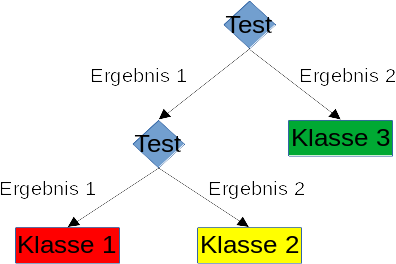
\includegraphics[width=0.5\linewidth]{images/entscheidungsbaum.png}
    \caption{Beispiel eines binären Entscheidungsbaums mit 3 möglichen Ergebnissen.}
    \label{fig:entscheidungsbaum}
\end{figure}
Das Trainieren von Entscheidungsbäumen ist eine Art von \textit{Supervised Learning}, d. h. aus einer beschrifteten Trainingsmenge werden Regeln abgeleitet, um das korrekte Mapping von Input
zu Output abzubilden \cite{goshKMeans}. Die Trainingsmenge besteht aus Feature-Mengen, die mit Klassen beschriftet sind \cite{steinbergCART}. Die Generalisierungsfähigkeit ist abhängig von der
Trainingsmenge. Zum einen sollte die Trainingsmenge möglichst repräsentativ sein für die Aufgabe, die gelernt werden soll. Zum anderen sollten die verwendeten Features eine Partitionierung
aller Klassen ermöglichen \cite{pei1998feature}.
\newline
\newline
Entscheidungsbäume werden heuristisch konstruiert, da die Konstruktion eines optimalen Entscheidungsbaumes NP-Vollständig ist \cite{laurent1976constructing}. Zu diesen Algorithmen gehören
beispielsweise \texttt{ID3} \cite{quinlan1986induction}, \texttt{C4.5} \cite{quinlan2014c4} oder \texttt{CART} \cite{breiman1984classification}. Die Aufgabe ist durch gezielte Trennungen
eine Partitionierung der Trainingsmenge zu erzeugen, sodass möglichst nur Einträge mit der gleichen Beschriftung in einer Partitionierung enthalten sind. Die Algorithmen unterscheiden
sich in ihrer Strategie \cite{quinlan1986induction}.
\newline
\newline
Scikit-Learn implementiert eine optimierte Version des \textit{CART} (\textbf{C}lassification \textbf{A}nd \textbf{R}egression \textbf{T}rees) Algorithmus \cite{ScikitLearnCART}.
CART partitioniert die Trainingsmenge indem lokal immer die beste Teilung ausgewählt wird, d. h. es wird für die momentane Teilmenge immer die beste Teilungsregel ausgewählt.
Dieser Vorgang wird rekursiv mit jeder Teilmenge wiederholt, bis keine weitere Teilung mehr möglich ist oder alle Einträge einer Partitionierung die gleiche Beschriftung tragen \cite{steinbergCART}.
\section{Ensemble-Methoden}
\label{sec:dt_ensemble_methods}
Ensemble-Methoden beschreiben wie mehrere Entscheidungsbäume trainiert werden, um eine möglichst hohe Diversität der einzelnen Entscheidungsbäume zu erzielen. Das Ergebnis eines Ensembles
ist die Aggregation der Ergebnisse der einzelnen Entscheidungsbäume \cite{dietterich2002ensemble}.
\newline
\newline
Der Wahlklassifizierer $H(x) = w_1 h_1(x) + ... + w_K h_K(x)$ ist eine Möglichkeit die Einzelergebnisse $\{h_1, ..., h_K\}$ gewichtet mit $\{w_1, ..., w_K\}$ zu aggregieren \cite{dietterich2002ensemble}.
Ein Ergebnis kann auf zwei Arten modelliert sein.
Einerseits als eine Funktion $h_i: D^n \mapsto \setR^m$, die einer $n$-dimensionalen Menge $D^n$ jeder der $m$ möglichen Klassen eine Wahrscheinlichkeit zuweist.
Das Ergebnis ist eine Wahrscheinlichkeitsverteilung.
Das diskrete Ergebnis der Klassifizierung ist die Klasse mit der höchsten Wahrscheinlichkeit in dem Ergebnis.
Alternativ kann es als eine Funktion $h_i: D^n \mapsto M$ abgebildet werden, die diskret auf eine der möglichen Klassen in $M$ verweist \cite{dymelThesis}.
In diesem Fall wird die Klasse ausgewählt, die am häufigsten unter allen Einzelergebnissen vorkam.
In der Praxis wird die Aggregation der Wahrscheinlichkeitsverteilung genutzt \cite{ScikitLearnEnsemble}.
Analog ist $H: D^n \mapsto \setR^m$ oder $H: D^n \mapsto M$ definiert \cite{dietterich2002ensemble}.
Für gewöhnlich hat jeder Teilnehmer einer Wahl das gleiche Gewicht.
\newline
\newline
Bagging (\textbf{B}ootstrap \textbf{agg}regat\textbf{ing}) konstruiert Entscheidungswälder, indem es Entscheidungsbäume mit Teilmengen der Trainingsmenge trainiert.
Abbildung \ref{fig:bagging} illustriert die Bagging Methode für $n$ Entscheidungsbaummodelle. Zunächst wird die Trainingsmenge in $n$ Teilmengen aufgeteilt \cite{breiman1996bagging}.
Der Inhalt der Teilmengen wird mit der \glqq Bootstrap sampling\grqq\ Methode bestimmt. Diese zieht aus einer Grundmenge $l$-mal jeweils $k$-Einträge \cite{efron1992bootstrap}.
Mit jeder Teilmenge wird ein Entscheidungsbaum trainiert \cite{breiman1996bagging}. Die Einzelergebnisse werden aggregiert, z. B. mit dem Wahlklassifizierer.
\begin{figure}[h!]
    \centering
    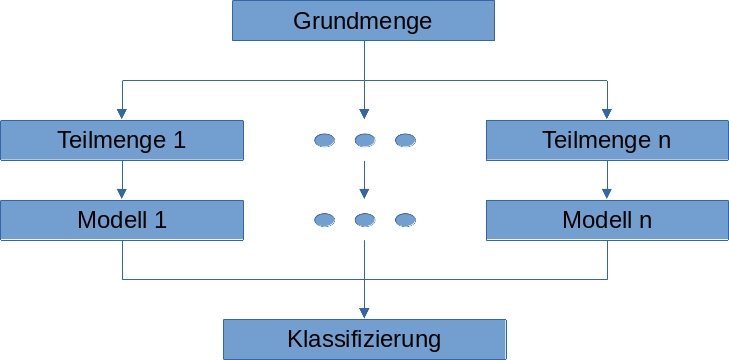
\includegraphics[width=0.6\linewidth]{images/bagging.jpg}
    \caption{Klassifizierungsprozess mit der Bagging-Methode.}
    \label{fig:bagging}
\end{figure}
\newline
\newline
Random Forest erweitert die Bagging-Methode \cite{breiman2001random}. Für jeden Entscheidungsbaum der trainiert werden soll, wird zusätzlich zufällig eine Teilmenge der Feature-Menge ausgewählt.
\newline
\newline
Extremely Randomized Trees (ExtraTrees) verwenden ebenfalls eine Teilmenge der Feature-Menge der Trainingsmenge beim Trainieren der einzelnen Entscheidungsbäume \cite{geurts2006extremely}.
Allerdings wird für jeden Entscheidungsbaum die gesamte Trainingsmenge verwendet. Bei der Konstruktion wird nicht versucht die beste Teilungsregel zu finden,
sondern es werden zufällig Teilungsregeln generiert, aus denen die Beste ausgewählt wird.
\newline
\newline
Beim Boosting werden nacheinander schwache Lerner auf einer Teilmenge trainiert, die gewichtet aggregiert werden \cite{freund1997decision}. Dadurch entsteht ein starker Lerner.
Abbildung \ref{fig:boosting} illustriert, wie vier schwache Lerner trainiert werden. Jeder Lerner findet eine Funktion der die trainierte Teilmenge unterteilt. Anschließend
werden sie gewichtet aggregiert. Dies konstruiert einen starken Lerner, der die gesamte Trainingsmenge unterteilt.
Diese Arbeit verwendet für Boosting den Algorithmus \texttt{AdaBoost} \cite{freund1997decision} von Freund und Schapire.
\begin{figure}[h!]
    \centering
    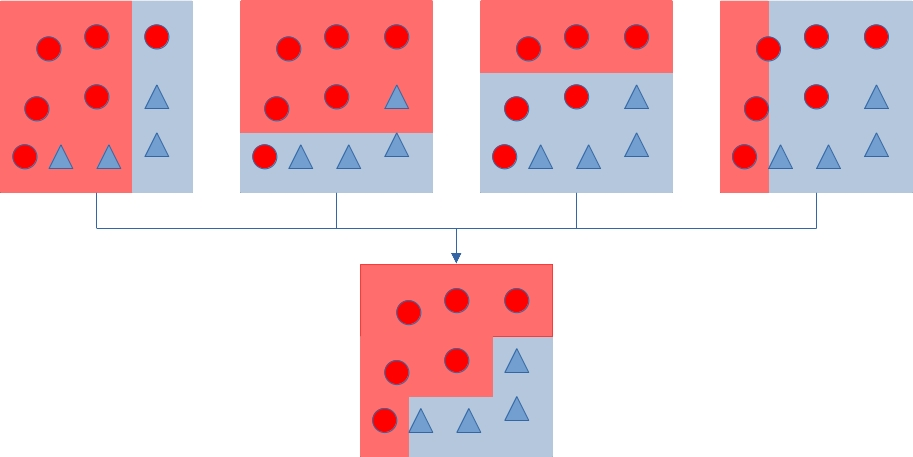
\includegraphics[width=\linewidth]{images/boosting.jpg}
    \caption{Klassifizierungsprozess mit der Boosting-Methode.}
    \label{fig:boosting}
\end{figure}
\section{Cherry-Picking}
\begin{itemize}
    \item Gehe hier auf Monte Carlo etc ein.
\end{itemize}
\section{Ressourcenbedarf auf dem Mikrocontroller}
\label{sec:dt_resource_usage}
Zukünftig soll das Modell auf einem Mikrocontroller ausgeführt werden \cite{antragForschungsprojekt}.
Mikrocontroller sind stark limitiert in ihrer Rechenleistung, Speicherkapazität, RAM und werden oft zudem mit einer Batterie betrieben.
Aus diesem Grund ist der Energieverbrauch zu minimieren und das Modell muss innerhalb dieser Limitierungen operieren können.

\newpage
\subsection{Ausführungszeit und Energieverbrauch}
\label{sub_sec:dt_ru_execution_time}
Der Energieverbrauch korreliert mit der Ausführungszeit.
Je länger die CPU ausgeschaltet ist, desto weniger Energie wird verbraucht.
Kurze Ausführungszeiträume vergrößern den Zeitraum, in dem die CPU ausgeschaltet sein kann.
Die Ausführungszeit ist die Zeit die benötigt wird, um alle Instruktionen auszuführen \cite{dymelThesis}.
Jede Instruktion bedarf eine bestimmte Anzahl an CPU-Zyklen.
Die Zeit pro Zyklus ist abhängig von der Taktrate der CPU.
\newline
\newline
Die Ausführungszeit eines Entscheidungswaldes setzt sich zusammen aus der Zeit für die Feature-Extrahierung, der Evaluierung aller im Ensemble enthaltenen Entscheidungsbäume
und der Aggregierungsfunktion.
Im schlimmsten Fall muss die gesamte Höhe eines Entscheidungsbaumes traversiert werden, um das Ergebnis zu bestimmen. Aus diesem Grund skaliert die Ausführungszeit mit der
traversierten Höhe jedes Baumes.
\newline
\newline
Um die Instruktionen zu minimieren sollten Datentypen verwendet werden, die von der CPU mit höchstens einem Wort dargestellt werden können.
Eine 8-Bit CPU würde zum Laden in Register eines 32-Bit Datentypen vier mal so viele Instruktionen benötigen wie bei einem 8-Bit Datentypen.
Außerdem sollten Operationen verwendet werden, die durch native Hardware-Operationen abgebildet werden können.
Ist dem nicht so, muss diese Operation durch Software ersetzt werden.
Dies erfordert mehr Zyklen als eine native Operation in Hardware.
\newline
\newline
Zu Beachten bei der Minimierung ist, dass Instruktionen unterschiedlich viele Zyklen benötigen und Funktionsaufrufe Overhead erzeugen.
Ein Beispiel dafür ist die Optimierung \textit{Function Inlining} \cite{leupers1999function}.
Der Aufruf von Funktionen kann einen hohen Overhead durch den Kontextwechsel erzeugen.
Aus diesem Grund verringert diese Optimierung die Ausführungszeit, erhöht aber die die Programmgröße signifikant.
Im Umkehrschluss könnten durch die Verwendung von Funktionen der nutzen des Programmspeichers verringert werden, Ausführungszeit und Energieverbrauch aber erhöht werden.

\newpage
\subsection{Programmgröße}
\label{sub_sec:dt_ru_programm_size}
Die Programmgröße ist die Gesamtheit aller Instruktionen die für das Programm benötigt werden \cite{dymelThesis}.
Dabei ist der Anteil für die Entscheidungswälder integral und der Anteil für die perifären Funktionalitäten zu vernachlässigen.
Die Programmgröße, die für einen Entscheidungswald benötigt wird, skaliert mit der Waldgröße und Höhe der einzelnen Entscheidungsbäume.
\newline
\newline
Die Höhe des Entscheidungsbaumes ist die Verzweigungstiefe der verschachtelten Tests.
Jeder Test ist ein Vergleich mit einem Schwellenwert.
Die Programmgröße für einen Vergleich setzt sich zusammen aus den Operationen um die Operanden in die Register zu laden
und die Instruktion um den Vergleich durchzuführen, sowie Abzweiginstruktionen. Wie in Kapitel \ref{sub_sec:dt_ru_execution_time}
sind Instruktionen durch einen passenden Datentypen zu vermeiden.
\newline
\newline
Ein weiterer Faktor sind die Instruktionen, die zur Rückgabe des Klassifizierungsergebnis benötigt werden.
In Kapitel \ref{sec:dt_ensemble_methods} wurden verschiedene Möglichkeiten der Rückgabe diskutiert, die relevant bei dem Aggregierungsprozess eines Ensembles ist.
Einerseits kann die Rückgabe eine Wahrscheinlichkeitsverteilung sein und andererseits eine diskrete Klasse.
Bei $m$ möglichen Klassen würde die erste Variante $m$-mal so viele Instruktion benötigen, wie die zweite Variante, da der Rückgabevektor zuvor mit der Wahrscheinlichkeitsverteilung gefüllt werden muss.
In der Praxis werden aber weniger Instruktion benötigt, da es eine große Überschneidung der Wahrscheinlichkeitsverteilungen gibt, die zurück gegeben werden.
Die Instruktionen, um den Rückgabevektor zu befüllen, können durch \textit{Basic Blocks}, d. h. beschriftete Instruktionsblöcke, geschickt recycled werden.
Zudem können Zuweisungen ausgelassen werden, die die Wahrscheinlichkeit 0 zuweisen, da der Vektor mit Nullen initialisiert wird.
Dennoch werden signifikant mehr Instruktionen benötigt als bei der diskreten Variante.
Aus diesem Grund wurde ein hybrider Ansatz vorgeschlagen, der im Falle eines eindeutigen Ergebnisses mit einer Toleranz von $\epsilon\in [0, 1]$ die diskrete Klasse statt der Wahrscheinlichkeitsverteilung zurück gibt.

\chapter{Künstliche Neuronale Netze}
Das mathematische Modell von künstlichen neuronalen Netzen wurde von McCulloch und Pitts im Jahre 1943 erfunden \cite{mcculloch1943logical}.
Dieses Modell ist eine Abstraktion des biologischen Neuronen als logischer Mechanismus.
\newline
\newline
Das Nervensystem besteht aus einem Netz von Neuronen, die miteinander verbunden sind und über elektrische Impulse miteinander interagieren \cite{rosenblatt1961principles}.
Man unterscheidet beim biologischen Neuronen zwischen \textit{Afferent}-Neuronen, \textit{Efferent}-Neuronen und \textit{Inter}-Neuronen.
Afferent-Neuronen nehmen elektrische Signale von Organen entgegen und können als \textit{Input} interpretiert werden.
Efferent-Neuronen geben elektrische Signale an \textit{Effektorzellen} weiter und können als \textit{Output} interpretiert werden.
Inter-Neuronen nehmen elektrische Signale von Afferent-Neuronen oder Inter-Neuronen entgegen und geben sie an Inter-Neuronen oder Efferent-Neuronen weiter.
Wenn der Schwellenwert eines \textit{Dendrite} von einem Neuronen durch ein elektrisches Signal erreicht wurde, wird ein elektrisches Signal über den \textit{Axon} an ein
anderes Neuron oder Effektorzellen übertragen.
\newline
\newline
Diese Charakteristiken werden mathematisch als ein Vergleich von einer gewichtete Summe von eingehenden Signalen mit einem Schwellenwert modelliert \cite{higham2019deep}.
Dieser Zusammenhang wird durch (\ref{formular:neuron_activation}) formalisiert.
\begin{align}
    \label{formular:neuron_activation}
    y = \sigma(\sum_{i=1}^n\textbf{w}_i\textbf{x}_i + b)
\end{align}
Die Vergleichsoperation ist die \textit{Aktivierungsfunktion} $\sigma: \mathbb{R}\mapsto\mathbb{R}$, die in diesem Fall die Stufenfunktion ist.
Die Eingabe $\textbf{x}\in\mathbb{R}^n$ wird mit $\textbf{w}\in[0, 1]^n$ gewichtet und der \textit{Bias} $b\in\mathbb{R}$ wird addiert. Der Bias stellt den Schwellenwert dar.
\newpage
Das künstliche neuronale Netz approximiert eine arbiträre Funktion $f^*$. Dazu findet es eine Menge von Parametern $\boldsymbol\theta$, wodurch $f^*(\textbf{x})\approx f(\textbf{x}, \boldsymbol\theta)$
möglichst gut von der Approximationsfunktion $f$ abgebildet wird \cite{bengio2017deep}.
\newline
\newline
Das KNN ist in Schichten organisiert. Analog zu den biologischen Neuron, gibt es eine \textit{Eingabeschicht (engl. Input-Layer)},
\textit{Ausgabeschicht (engl. Output-Layer)} und \textit{verdeckte Schichten (engl. Hidden-Layer)}.
Dies wird in Abbildung \ref{fig:neural_network_example} illustriert.
Analog zur Aktivierung eines einzelnen Neuronen, dargestellt in (\ref{formular:neuron_activation}), stellt
(\ref{formular:layer_activation}) die Aktivierung einer Schicht dar \cite{higham2019deep}.
\begin{align}
    \label{formular:layer_activation}
    \textbf{a}_{l} = \sigma_l(\textbf{z}_l), \hspace{2cm} \textbf{z}_l := \textbf{W}_l\textbf{a}_{l-1} + \textbf{b}_l
\end{align}
\begin{figure}[h!]
    \centering
    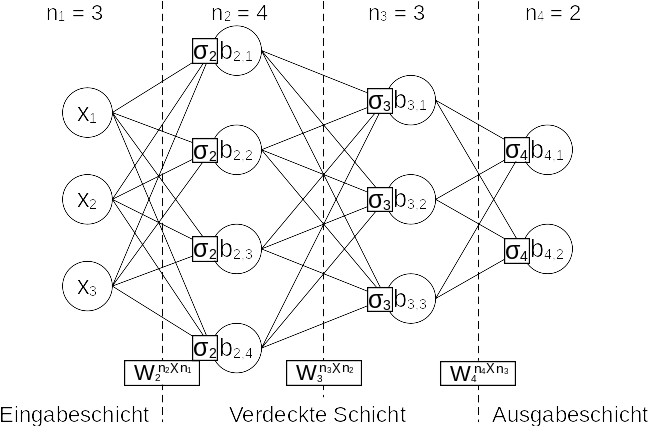
\includegraphics[width=0.8\linewidth]{images/neural_network_example.png}
    \caption{Beispiel eines FFNN mit vier Schichten und einer binären Ausgabeschicht.}
    \label{fig:neural_network_example}
\end{figure}
\newline
Das allgemeine KNN verfügt über $L\in\mathbb{N}$ Schichten. Jede Schicht $l$ verfügt über $n_l\in\mathbb{N}$ Neuronen.
Die Aktivierungsfunktion $\sigma_l:\mathbb{R}^{n_{l}}\mapsto\mathbb{R}^{n_{l}}$ berechnet die Aktivierung mit der gewichteten Summe $\textbf{z}_l$.
Die gewichtete Summe setzt sich zusammen aus der Aktivierung der vorherigen Schicht $\textbf{a}_{l-1}$ die mit $W_i\in\mathbb{R}^{n_{l}\times{n_{l-1}}}$ gewichtet wird.
Die Schwellenwerte der Neuronen werden durch die Biase $\textbf{b}_l\in\mathbb{R}^{n_{l}}$ dargestellt.
In (\ref{formular:general_knn}) wird das allgemeine KNN mit einer rekursiven Funktion modelliert.
\begin{align}
    \label{formular:general_knn}
    \textbf{a}_1 := \textbf{x}, \hspace{1cm}
    \textbf{z}_l := \textbf{W}_l\textbf{a}_{l-1} + \textbf{b}_l, \hspace{1cm}
    \textbf{a}_l := \sigma_l(\textbf{z}_l), \hspace{1cm} \textbf{f(x)} := \textbf{a}_L
\end{align}
\newpage
Diese Arbeit nutzt ausschließlich \textit{Feed Forward neuronale Netzwerke}.
Diese werden durch \textit{dichte Schichten (engl. Dense-Layer)} charakterisiert, d. h. Schichten in denen alle Neuronen
einer Schicht mit allen Neuronen der folgenden Schicht verbunden sind \cite{bengio2017deep}.

\section{Keras}
Keras ist die am meisten genutzte \textit{deep learning} API und wurde in Python geschrieben \cite{kerasDoc}.
Dadurch ist sie kompatibel mit allen gängigen Betriebssystemen.
Ihr Fokus ist eine intuitive und simple API anzubieten, sodass schnelle Iterationen im Entwicklungsprozess möglich sind.
Trotzdem ist sie effizient und skalierbar, um die Kapazitäten großer Rechenverbunde auszunutzen.
\newline
\newline
Keras abstrahiert das ML System \textit{Tensorflow}. Tensorflow implementiert ML Algorithmen, die dem Stand der Forschung entsprechen.
Der Fokus ist auf effizientes Training der Modelle \cite{abadi2016tensorflow} gerichtet.
Dafür nutzt es die Multikernarchitektur von CPUs, GPUs und spezialisierter Hardware, sogenannten TPUs (\textbf{T}ensor \textbf{P}rocessing \textbf{U}nit), aus.
Es wurde als open-source Projekt veröffentlicht und ist weit verbreitet.
\newline
\newline
Keras bietet die in dieser Arbeit benötigten Algorithmen an, weshalb es zum Trainieren von FFNNs verwendet wird.
\section{Training der ML-Modelle}
\label{sec:model_training}
Typischerweise haben weder Entscheidungsbaum basierte Klassifizierer noch FFNNs Rückwärtskanten.
Neuronale Netze mit Rückwärtskanten werden als \textit{rekurrente Netze} (RNN) bezeichnet.
Abbildung \ref{fig:model_idea} zeigt, dass die Rückwärtskante genutzt wird, um das Klassifizierungsergebnis,
also den vorherigen Standort, bei der Feature-Extrahierung zu nutzen.
Das Klassifizierungsergebnis ist aber nicht immer korrekt, wodurch fehlerhafte Features im Zusammenhang
mit dem Klassifizierungsergebnis als Eingabe in das ML-Modell verwendet werden können.
Damit das ML-Modell lernt mit diesem Fehler umzugehen, ist es notwendig, dass das ML-Modell Trainingsbeispiele mit
Features auf Basis eigener Klassifizierungsbeispiele zur Verfügung hat.
\newline
\newline
Abbildung \ref{fig:training_explained} illustriert den Trainingsablauf.
Die simulierten Daten der aufgenommenen Routen sind unterteilt in Partitionen basierend auf deren Zyklusbeschriftung,
damit in jeder Partition alle Standorte vorhanden sind.
Der Zyklus ist ein Umlauf einer Route, bevor sie wiederholt wird.
Insgesamt besteht die Datenmenge aus 20 Zyklen.
Die ersten fünf Zyklen werden zum \glqq Aufwärmen \grqq\ verwendet,
d. h. das ML-Modell wird mit korrekt beschrifteten Daten trainiert, welche es nicht selbst beschriftet hat.
In den folgenden zehn Zyklen werden weitere Partitionen zur Trainingsmenge hinzugefügt, die mit quadratisch steigendem Anteil vom ML-Modell selbst beschriftet sind.
Zunächst werden 50\% der Partition $i$ vom ML-Modell beschriftet, bis beim 13. Zyklus schließlich 100\% beschriftet wird.
Die Elemente aus der Partition, die beschriftet werden sollen, sind zufällig, damit der Klassifizierungsfehler auf allen Teilstücken der Route gelernt werden kann.
\begin{figure}[h!]
    \centering
    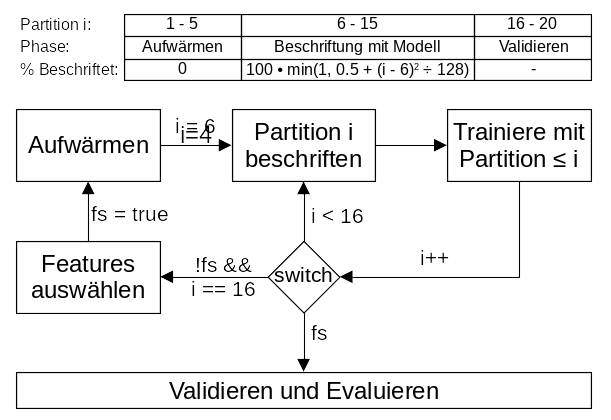
\includegraphics[width=\linewidth]{images/training_explained.png}
    \caption{Der Trainingsablauf des verfolgten Ansatzes.}
    \label{fig:training_explained}
\end{figure}
\newline
\newline
Die erste Trainingsphase ist abgeschlossen, nachdem das ML-Modell mit einer Trainingsmenge von 15 Zyklen trainiert wurde.
Anschließend wird einmalig eine Feature-Auswahl betrieben, in der insignifikante Features aus der Feature-Menge entfernt werden.
Features sind insignifikant, die eine geringe Wichtigkeit aufweisen (Kapitel \ref{sec:eval_feature_importance}).
Dies ermöglicht kleinere ML-Modelle zu verwenden und verringert die Dimensionen des Suchraumes, wodurch das Trainieren erleichtert wird.
Außerdem müssen Modelle individuell für verschiedene Einsatzgebiete trainiert werden, bei denen möglicherweise einige Sensoren bzw. Features nicht genutzt werden.
In Abbildung \ref{fig:training_explained} ist die Feature-Auswahl nur einmalig vorgesehen.
Denkbar wäre aber auch eine iterative Eliminierung der Features oder Optimierung durch ein evolutionären Algorithmus.
Anschließend wird das ML-Modell erneut auf den Partitionen trainiert, bis es validiert und evaluiert werden kann.
\newline
\newline
Die ML-Modelle ohne Rückwärtskante sind deutlich simpler.
Diese müssen nicht in Zyklen trainiert werden, sondern können direkt mit der vollständigen Trainingsmenge trainiert werden,
wodurch das Training deutlich effizienter ist.
\section{Optimierer}
Die Strategie im Optimierungsprozess wird als Optimierer bezeichnet.
Diese Algorithmen steuern, wie die Parameter $\boldsymbol\theta$ aktualisiert werden.
Die Eingabe sind die Kosten der Trainingsdaten.
Üblicherweise wird \textit{ADAM} verwendet.
ADAM ist eine Kombination aus \textit{SGD} (\textbf{S}tochastic \textbf{G}radient \textbf{D}escent) mit Momentum und \textit{RMSprop}.
\newline
\newline
SGD ist eine Approximation von \textit{Gradient Descent} (GD).
GD ist ein iterativer Algorithmus, der den Gradienten in Richtung des Extrema folgt und dementsprechend die Eingabeparameter aktualisiert.
\begin{align}
    \label{formular:gradient_descent}
    x_{k+1} := \begin{cases}
                   x_k - C^{\prime}(x_k)\alpha_k & \text{, wenn } C(x_k - C^{\prime}(x_k)\eta_k) < C(x_k)\\
                   (1 + \alpha_k)x_k & \text{, ansonsten}
    \end{cases}
\end{align}
Gleichung \ref{formular:gradient_descent} illustriert diesen iterativen Prozess für Minimierung im eindimensionalen Fall,
wobei $\eta_k > 0$ eine angemessene \textit{Lernrate} ist, $x$ der Eingabeparameter und $C$ die Kostenfunktion.
Ist die Lernrate zu groß könnte keine Verbesserung beobachtet werden, da das Maxima immer übersprungen wird.
Ist die Lernrate zu klein könnte die Konvergenz sehr langsam sein.
\newline
\newline
Im mehrdimensionalen Fall wird für jede Komponente des Eingabevektors dieser Prozess durchgeführt, sodass für jede Komponente
die Richtung des Extrema verfolgt wird.
Dies impliziert, dass GD sehr aufwendig zu berechnen ist für Eingabevektoren mit hohen Dimensionen.
Gleichung \ref{formular:gd_multi_dim} zeigt die iterative Berechnung im mehrdimensionalen Fall.
\begin{align}
    \label{formular:gd_multi_dim}
    \textbf{x}_{k+1} = \textbf{x}_k - \bigtriangledown C(\textbf{x}_k)\eta_k
\end{align}
Zur Berechnung muss der Gradient des Eingabevektors berechnet werden.
Je größer die Dimension des Eingabevektor ist, desto aufwendiger ist die Berechnung.
\newline
\newline
SGD nimmt an, dass eine Verbesserung wahrscheinlich ist, wenn eine Komponente, bzw. ein \textit{mini-batch} (Teilmenge), des
Eingabevektors in Richtung des Extrema aktualisiert wird.
Aus diesem Grund werden die Parameter aktualisiert, nachdem jeweils nur eine Komponente des Eingabevektors aktualisiert wurde.
Dadurch bedarf das neuronale Netzwerk zur Konvergenz mehr Epochen, muss aber weniger Berechnungen durchführen.
\newline
\newline
(S)GD mit Momentum versucht zu vermeiden, dass lokale Extrema gefunden werden anstatt globale Extrema, indem Momentum aus
vorherigen Gradienten beibehalten wird, um aus lokalen Extrema wieder raus zu finden.
Gleichung \ref{formular:sgd_momentum} zeigt die iterative Berechnung.
\begin{align}
    \label{formular:sgd_momentum}
    \textbf{v}_{-1} = \textbf{0}, \hspace{0.6cm} \textbf{v}_k = \textbf{v}_{k-1}\gamma +
    \bigtriangledown f(\textbf{x}_k), \hspace{0.6cm} \textbf{x}_{k+1} = \textbf{x}_k - \textbf{v}_k\eta
\end{align}
Zur Berechnung wird ein Hilfsvektor $\textbf{v}$ verwendet, welcher das Momentum vergangener Gradienten darstellt.
In jeder Iteration fließt ein Anteil $\gamma$, typischerweise $\gamma=0.9$, von dem Hilfsvektor in die Berechnung der neuen Eingabeparameter ein.
Der Unterschied zum GD (\ref{formular:gd_multi_dim}) ist der Anteil vergangener Gradienten.
\newline
\newline
RMSprop ist eine Variante von \textit{Adagrad}.
Adagrad passt die Lernrate $\eta$ an, denn typischerweise wird zuerst eine hohe Lernrate benötigt und je näher sich dem Extrema angenähert wird,
sollte diese Lernrate sinken.
Gleichung \ref{formular:adagrad} zeigt, wie sich iterativ die Lernrate antiproportional
zur kummulierten Norm der Gradienten der Kostenfunktion verringert.
Dabei wird für $\epsilon$ eine kleine Zahl gewählt, um Teilen durch 0 zu vermeiden aber keinen signifikanten Einfluss auf die Berechnung zu haben.
\begin{align}
    \label{formular:adagrad}
    \textbf{g}_k = \bigtriangledown C_{j_k}(\textbf{x}_k), \hspace{0.6cm}
    \textbf{w}_k = \textbf{w}_{k-1} + \textbf{g}_k^2, \hspace{0.6cm}
    \textbf{x}_{k+1} = \textbf{x}_k - \textbf{g}_k \circ \frac{\eta}{\sqrt{\textbf{w}_k + \epsilon}}
\end{align}
Das Problem an Adagrad ist, dass die Lernrate zu schnell gegen 0 konvergieren kann, wodurch das Zielextrema nicht erreicht wird.
RMSprop (\ref{formular:rmsprop}) löst dieses Problem, indem in jeder Iteration ein Zerfallsfaktor $\gamma < 1$ auf den Hilfsvektor $\textbf{w}$ angewendet wird
und Anteilweise das Hadamard-Produkt des Gradienten der Kostenfunktion addiert wird.
\begin{align}
    \label{formular:rmsprop}
    \textbf{w}_{-1} = \textbf{0}, \hspace{0.6cm}
    \textbf{g}_k = \bigtriangledown C_{j_k}(\textbf{x}_k), \hspace{2cm} \nonumber\\
    \textbf{w}_k = \textbf{w}_{k-1}\gamma + \textbf{g}_k^2 (1-\gamma), \hspace{0.6cm}
    \textbf{x}_{k+1} = \textbf{x}_k - \textbf{g}_k \circ \frac{\eta}{\sqrt{\textbf{w}_k + \epsilon}}
\end{align}
Gleichung \ref{formular:adam} zeigt, wie Adam RMSprop und SGD mit Momentum vereint, wobei $\gamma_1 < \gamma_2 < 1$.
Adam nutzt zwei Hilfsvektoren $\textbf{v}$ und $\textbf{w}$, die mit einer Zerfallsrate wachsen und beim Lernen
sowohl Momentum nutzt, um lokale Extrema zu überbrücken, und passt die Lernrate im Laufe des Trainingsprozesses an.
\begin{align}
    \label{formular:adam}
    \textbf{v}_{-1} = \textbf{w}_{-1} = \textbf{0}, \hspace{3.5cm} \nonumber\\
    \textbf{g}_k = \bigtriangledown C_{j_k}(\textbf{x}_k), \hspace{0.6cm}
    \textbf{v}_k = \textbf{v}_{k-1}\gamma_1 + \textbf{g}_k (1-\gamma_1), \hspace{1cm} \nonumber\\
    \textbf{w}_k = \textbf{w}_{k-1}\gamma_2 + \textbf{g}_k^2 (1-\gamma_2), \hspace{0.6cm}
    \textbf{x}_{k+1} = \textbf{x}_k - \textbf{v}_k \circ \frac{\eta}{\sqrt{\textbf{w}_k + \epsilon}}
\end{align}
\section{Aktivierungsfunktionen}
Die Aktivierungsfunktion entscheided ob ein Neuron aktiviert wird oder nicht \cite{nwankpa2018activation}.
Sie können entweder linear oder nicht-linear sein.
Es ist aber nötig nicht-lineare Funktionen zu verwenden, damit jede kontinuierliche Funktion approximiert werden kann \cite{apicella2021survey}.
Sie unterscheiden sich in ihren Eigenschaften und Berechnungskosten, was eine besondere Rolle für Mikrocontroller spielt.
\newline
\newline
In der frühen Geschichte der neuronalen Netzwerke wurde die \textit{Sigmoid}-Funktion (\ref{formular:af_sigmoid}) viel verwendet, da sie asymptotisch begrenzt,
kontinuierlich und nicht-linear ist \cite{apicella2021survey}.
Oft wird sie heute in der Ausgabeschicht für binäre Klassifizierungsprobleme eingesetzt \cite{nwankpa2018activation}.
Allerdings ist sie für tiefe neuronale Netzwerke ungeeignet, da der Gradient zwischen 0 und 0.25 ist und dadurch im
Backpropagation-Prozess bereits nach wenigen Schichten gegen 0 geht.
Die \textit{SoftMax}-Funktion (\ref{formular:af_softmax}) oder normalisierte Exponentialfunktion berechnet für einen Eingabevektor eine Wahrscheinlichkeitsverteilung.
Die Einträge dieser Verteilung können für die Wahrscheinlichkeiten der einzelnen Klassen eines multivariat Klassifizierungsproblem interpretiert werden.
\begin{align}
    \label{formular:af_sigmoid}
    \text{sigmoid}(x) = \frac{1}{1 + e^{-x}}
\end{align}
\begin{align}
    \label{formular:af_softmax}
    \text{softmax}(x_i) = \frac{e^{x_i}}{\sum_j e^{x_j}}
\end{align}
\subfigbox{
\subfigure[Sigmoid/SoftMax]{\label{subfig:af_sigmoid}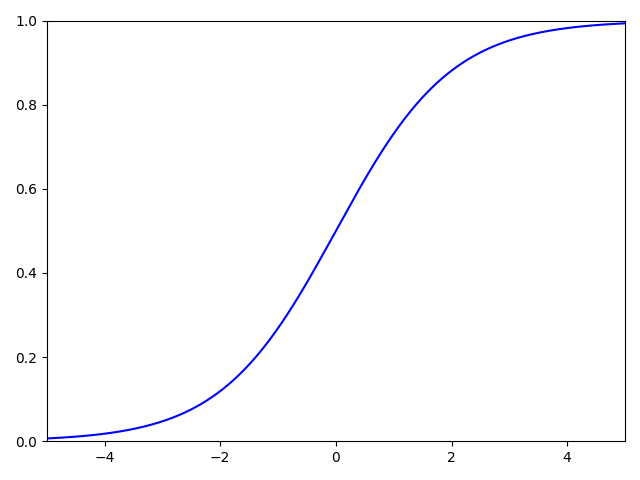
\includegraphics[width=0.495\linewidth]{images/activation_function_heaviside.png}}\hfill%
\subfigure[ReLU Varianten]{\label{subfig:af_relu}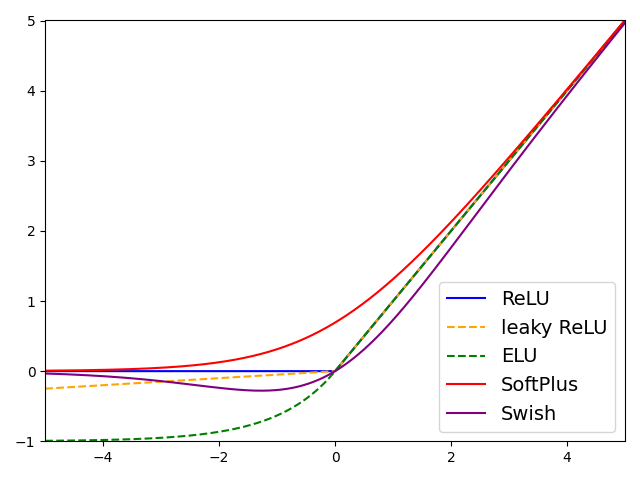
\includegraphics[width=0.495\linewidth]{images/activation_function_relu_varianten.png}}
}{Verschiedene Aktivierungsfunktionen.}{fig:activation_functions}
\newline
\newline
Zur \textit{ReLU}-Familie \cite{apicella2021survey} gehört die ReLU-Funktion \cite{glorot2011deep, konda2014zero, elfwing2018sigmoid, alcaide2018swish} und
ihre Varianten \cite{maas2013rectifier}, sowie die \textit{SoftPlus}- \cite{dugas2001incorporating} und \textit{Swish}-Funktion \cite{ramachandran2017searching}.
ReLU (\ref{formular:af_relu}) steht für \glqq\textit{rectified linear function}\grqq\ und wird häufig in modernen neuronalen Netzwerken verwendet \cite{apicella2021survey}.
Sie ist nicht differenzierbar bei 0 und die Ableitung für negative Eingaben ist 0.
Dies kann zu \textit{sterbenden Neuronen (engl. dying neurons)} führen, da der Bias so negativ wird, sodass das Neuron nicht mehr aktiviert wird.
Zudem ist der Trainingsprozess verlangsamt, wenn der Gradient konstant 0 ist.
Dafür ist die Ableitung der Funktion ansonsten 1, was den Backpropagation-Prozess vereinfacht, da der Gradient neutral zur Aktivierungsfunktion ist.
\begin{align}
    \label{formular:af_relu}
    \text{ReLU}(x) = \max(x, 0)
\end{align}
Varianten sind beispielsweise \textit{leaky ReLU} \cite{maas2013rectifier} (\ref{formular:af_leaky_relu}) und \textit{ELU (exponential linear unit)} (\ref{formular:af_elu})
\cite{clevert2015fast}, welche versuchen die Defizite des konstanten 0 Gradienten zu lösen, indem der negative Teil der Funktion nicht 0 ist.
\begin{align}
    \label{formular:af_leaky_relu}
    \text{leaky\_ReLU}_{\alpha}(x) = \begin{cases}
                               x & \text{, wenn } x \geq 0\\
                               \alpha x & \text{, ansonsten } (\alpha\in \mathbb{R}_{0}^{+})
    \end{cases}
\end{align}
\begin{align}
    \label{formular:af_elu}
    \text{ELU}_{\alpha}(x) = \begin{cases}
                                 x & \text{, wenn } x \geq 0\\
                                 \alpha(e^{x} - 1) & \text{, ansonsten } (\alpha\in \mathbb{R}_{0}^{+})
    \end{cases}
\end{align}
\textit{SoftPlus} (\ref{formular:af_softplus}) ist analytisch, dafür im Vergleich zu ReLU aufwendiger zu berechnen ist\cite{apicella2021survey}.
\begin{align}
    \label{formular:af_softplus}
    \text{softplus}(x_i) = \ln(e^x + 1)
\end{align}
Eine weitere Variante ist \textit{Swish} \cite{ramachandran2017searching} (\ref{formular:af_swish}).
Sie ist analytisch aber nicht monoton.
Im Vergleich zu ReLU ist sie aufwendig zu berechnen.
Ihre Autoren behaupten aber, dass dadurch bessere Ergebnisse erzielt werden können, ohne andere Parameter zu ändern.
\begin{align}
    \label{formular:af_swish}
    \text{swish}(x_i) = \frac{xe^x}{e^x + 1}
\end{align}
\section{Ressourcenbedarf auf dem Mikrocontroller}
\label{sec:dt_resource_usage}
Zukünftig soll das Modell auf einem Mikrocontroller ausgeführt werden \cite{antragForschungsprojekt}.
Mikrocontroller sind stark limitiert in ihrer Rechenleistung, Speicherkapazität, RAM und werden oft zudem mit einer Batterie betrieben.
Aus diesem Grund ist der Energieverbrauch zu minimieren und das Modell muss innerhalb dieser Limitierungen operieren können.

\newpage
\subsection{Ausführungszeit und Energieverbrauch}
\label{sub_sec:dt_ru_execution_time}
Der Energieverbrauch korreliert mit der Ausführungszeit.
Je länger die CPU ausgeschaltet ist, desto weniger Energie wird verbraucht.
Kurze Ausführungszeiträume vergrößern den Zeitraum, in dem die CPU ausgeschaltet sein kann.
Die Ausführungszeit ist die Zeit die benötigt wird, um alle Instruktionen auszuführen \cite{dymelThesis}.
Jede Instruktion bedarf eine bestimmte Anzahl an CPU-Zyklen.
Die Zeit pro Zyklus ist abhängig von der Taktrate der CPU.
\newline
\newline
Die Ausführungszeit eines Entscheidungswaldes setzt sich zusammen aus der Zeit für die Feature-Extrahierung, der Evaluierung aller im Ensemble enthaltenen Entscheidungsbäume
und der Aggregierungsfunktion.
Im schlimmsten Fall muss die gesamte Höhe eines Entscheidungsbaumes traversiert werden, um das Ergebnis zu bestimmen. Aus diesem Grund skaliert die Ausführungszeit mit der
traversierten Höhe jedes Baumes.
\newline
\newline
Um die Instruktionen zu minimieren sollten Datentypen verwendet werden, die von der CPU mit höchstens einem Wort dargestellt werden können.
Eine 8-Bit CPU würde zum Laden in Register eines 32-Bit Datentypen vier mal so viele Instruktionen benötigen wie bei einem 8-Bit Datentypen.
Außerdem sollten Operationen verwendet werden, die durch native Hardware-Operationen abgebildet werden können.
Ist dem nicht so, muss diese Operation durch Software ersetzt werden.
Dies erfordert mehr Zyklen als eine native Operation in Hardware.
\newline
\newline
Zu Beachten bei der Minimierung ist, dass Instruktionen unterschiedlich viele Zyklen benötigen und Funktionsaufrufe Overhead erzeugen.
Ein Beispiel dafür ist die Optimierung \textit{Function Inlining} \cite{leupers1999function}.
Der Aufruf von Funktionen kann einen hohen Overhead durch den Kontextwechsel erzeugen.
Aus diesem Grund verringert diese Optimierung die Ausführungszeit, erhöht aber die die Programmgröße signifikant.
Im Umkehrschluss könnten durch die Verwendung von Funktionen der nutzen des Programmspeichers verringert werden, Ausführungszeit und Energieverbrauch aber erhöht werden.

\newpage
\subsection{Programmgröße}
\label{sub_sec:dt_ru_programm_size}
Die Programmgröße ist die Gesamtheit aller Instruktionen die für das Programm benötigt werden \cite{dymelThesis}.
Dabei ist der Anteil für die Entscheidungswälder integral und der Anteil für die perifären Funktionalitäten zu vernachlässigen.
Die Programmgröße, die für einen Entscheidungswald benötigt wird, skaliert mit der Waldgröße und Höhe der einzelnen Entscheidungsbäume.
\newline
\newline
Die Höhe des Entscheidungsbaumes ist die Verzweigungstiefe der verschachtelten Tests.
Jeder Test ist ein Vergleich mit einem Schwellenwert.
Die Programmgröße für einen Vergleich setzt sich zusammen aus den Operationen um die Operanden in die Register zu laden
und die Instruktion um den Vergleich durchzuführen, sowie Abzweiginstruktionen. Wie in Kapitel \ref{sub_sec:dt_ru_execution_time}
sind Instruktionen durch einen passenden Datentypen zu vermeiden.
\newline
\newline
Ein weiterer Faktor sind die Instruktionen, die zur Rückgabe des Klassifizierungsergebnis benötigt werden.
In Kapitel \ref{sec:dt_ensemble_methods} wurden verschiedene Möglichkeiten der Rückgabe diskutiert, die relevant bei dem Aggregierungsprozess eines Ensembles ist.
Einerseits kann die Rückgabe eine Wahrscheinlichkeitsverteilung sein und andererseits eine diskrete Klasse.
Bei $m$ möglichen Klassen würde die erste Variante $m$-mal so viele Instruktion benötigen, wie die zweite Variante, da der Rückgabevektor zuvor mit der Wahrscheinlichkeitsverteilung gefüllt werden muss.
In der Praxis werden aber weniger Instruktion benötigt, da es eine große Überschneidung der Wahrscheinlichkeitsverteilungen gibt, die zurück gegeben werden.
Die Instruktionen, um den Rückgabevektor zu befüllen, können durch \textit{Basic Blocks}, d. h. beschriftete Instruktionsblöcke, geschickt recycled werden.
Zudem können Zuweisungen ausgelassen werden, die die Wahrscheinlichkeit 0 zuweisen, da der Vektor mit Nullen initialisiert wird.
Dennoch werden signifikant mehr Instruktionen benötigt als bei der diskreten Variante.
Aus diesem Grund wurde ein hybrider Ansatz vorgeschlagen, der im Falle eines eindeutigen Ergebnisses mit einer Toleranz von $\epsilon\in [0, 1]$ die diskrete Klasse statt der Wahrscheinlichkeitsverteilung zurück gibt.
\chapter{Standortbestimmung}
Als Standortbestimmung, oder \textit{Lokalisierung}, wird der Prozess bezeichnet die Position von einem Gerät oder Nutzer in einem Koordinatensystem zu bestimmen \cite{bulusu2000gps}.
Unterschieden wird dabei zwischen \textit{Indoor}- und \textit{Outdoor}-Lokalisierung \cite{zafari2019survey, bulusu2000gps}.
Bei Indoor-Lokalisierung wird ein Szenario innerhalb von Gebäuden betrachtet und bei Outdoor-Lokalisierung ein Szenario unter dem freien Himmel.
\newline
\newline
Weiterhin wird unterscheiden zwischen \textit{Device-Based}- und \textit{Device-Free}-Lokalisierung \cite{xiao2016survey}.
Bei Device-Based-Lokalisierung bestimmt das Gerät selbst die Position, wohingegen bei der Device-Free-Lokalisierung
die Position von der Infrastruktur bestimmt wird.
\newline
\newline
Lokalisierung ist aber nicht nur beschränkt für Geräte.
Menschen und Tiere haben einen Orientierungssinn, der die Navigation anhand von Orientierungspunkten ermöglicht \cite{menzel1996knowledge}.
Beispielsweise hängt die Navigation von Honigbienen stark von den Orientierungspunkten ab.
Anstatt die direkte Route zu wählen, fliegen Honigbienen die Orientierungspunkte ab, um zu ihrem Ziel zu gelangen.
Dabei ist die Navigation robust gegenüber leichte Veränderungen der Orientierungspunkte.

\section{Indoor- und Outdoor-Lokalisierung}
GPS ist eine weit verbreites Standortbestimmungssystem im Outdoor-Kontext  und kann für eine Vielzahl von Anwendungen eingesetzt werden,
z. B. Tracking, Navigation oder Rettungsaktionen \cite{kaplan2005understanding}.
Es skaliert zu einer arbiträren Anzahl von Nutzern, da es einen device-based Ansatz verwendet.
Die Geräte berechnen aus den empfangenden Signalen von mehreren Satelliten ihre Position.
Dabei ist die Standortbestimmung bis zu 5 m genau \cite{sadowski2018rssi},
wobei es Varianten gibt, die noch bessere Auflösungen erzielen können \cite{parkinson1996differential}.
Der Energieverbrauch ist sehr hoch \cite{jurdak2013energy}, wodurch es ungeeignet für kleine batteriegestützte Systeme ist.
In einem Indoor-Kontext kann GPS aber meistens nicht eingesetzt werden,
da das Gebäude die benötigte Signalstärke zu den Satteliten beeinträchtigen kann \cite{xiao2016survey, jin2006indoor}.
Aus diesem Grund ist es für batteriegestützte Mikrocontroller im Indoor-Bereich suboptimal.
\newline
\newline
Indoor-Lokalisierung bedarf meist einer hohen Auflösung, muss sicherheitskritische Vorgaben einhalten,
energieeffizient sein, skalierbar sein und geringe Kosten haben \cite{xiao2016survey}.
Es gibt verschiedene Ansätze, die entweder device-based oder device-free sind.
\newline
\newline
Device-based Ansätze nutzen die Sensoren des Geräts, um die Position zu bestimmen \cite{xiao2016survey}.
Beispielsweise können visuelle Features mit der Kamera extrahiert werden \cite{poulose2019hybrid, cunha2011using},
RSS Messungen des WiFi Netzwerkes durchgeführt werden \cite{pan2008transfer},
Bewegungs- oder Lichtsensoren verwendet werden \cite{poulose2019hybrid, wang2018deepml, xiao2016survey}.
Der Vorteil sind die geringen Infrastrukturkosten \cite{xiao2016survey}.
\newline
\newline
Device-free Ansätze bedürfen einer Infrastruktur, um Objekte im Interessebereich wahrzunehmen \cite{xiao2016survey}.
Diese werden zum Beispiel für Überwachsungsszenarien eingesetzt \cite{qian2018widar2}.
Ansätze nutzen beispielsweise die bestehende Kamerainfrastruktur aus \cite{kim2019info},
WiFi basierte Ansätze \cite{qian2018widar2}, Infrarot basierte Ansätze \cite{kemper2010passive}
oder RFID basierte Ansätze \cite{yang2015see}.
\newpage
\section{WiFi basierte Indoor-Lokalisierung mit Transfer Lernen}
Pan et al. untersuchten Indoor-Lokaliserung basierend auf WiFi RSS Daten \cite{pan2008transfer}.
Der Empfänger misst die \textit{Received Signal Strength} (RSS) mehrerer Sender.
Dadurch steht ein Vektor von Signalstärken zur Verfügung aus dem die Position approximiert werden kann.
\newline
\newline
Pan et al. stellen fest, dass bei ML Ansätzen oft zwei Annahmen getroffen werden.
Zum einen wird eine \textit{Offline}-Phase vorausgesetzt mit ausreichend beschrifteten Daten,
d. h. eine Trainingsphase bevor das Modell eingesetzt wird.
Zum anderen wird angenommen, dass das gelernte Modell statisch über Zeit, Raum und Geräte ist.
\newline
\newline
In der Praxis können sich Modelle jedoch über die Zeit ändern, z.~B. wenn Mitarbeiter Mittags zur Kantine gehen.
Es kann schwierig sein ausreichend Daten für große Gebäude zu sammeln.
Verschiedene Geräte können verschiedene Sensorwerte erfassen.
Dies führt zu einen erheblichen Kalibrierungsaufwand der ML Modelle.
\newline
\newline
Pan et al. schlagen Transfer Learning vor, um dieses Problem zu lösen.
Transfer Learning befasst sich mit dem Problem, wenn Trainings- und Testdaten verschiedener Verteilungen folgen oder in verschiedenen Feature-Räumen repräsentiert sind.
Die gewonnene Erfahrung beim Training soll dabei auf das neue, ähnliche Problem übertragen werden.
Dafür müssen Beziehungen gefunden werden, die den Erfahrungstransfer ermöglichen.
\newline
\newline
Sie trainierten ein \textit{Hidden Markov Model} (HMM), wobei die Ortserkennung als Klassifizierungsproblem diskreter Orte modelliert wurde.
Auf ihren Testdaten waren sie signifikant besser als Ansätze ohne Transfer Learning.

\section{Indoor-Lokalisierung mit Magnet- und Lichtsensoren}
Wang et al. haben einen Indoor-Lokalisierungsansatz untersucht, der Magnetfelddaten und
Lichtsensordaten eines Smartphones nutzt, um die Position des Gerätes zu bestimmen \cite{wang2018deepml}.
In einem Vorverarbeitungsschritt kombinieren die Autoren Magnetfelddaten und Lichsensordaten.
Damit wird ein Deep LSTM (\textbf{L}ong  \textbf{S}hort \textbf{T}erm \textbf{M}emory NN) trainiert.
\newline
\newline
Die Autoren merken an, dass viele Ansätze RSS oder CSI (\textbf{C}hannel \textbf{S}tate \textbf{I}nformation) nutzen, um Indoor-Lokalisierungsmodelle zu generieren.
Diese sind aber unzerverlässig, wenn die Signalstärke schlecht ist oder nicht verfügbar, z. B. in einem Parkhaus.
Dahingegen ist das Magnetfeld und Licht omnipresent.
Die Magnetfelddaten weisen eine geringe Varianz auf.
Diskrete Orte können aber durch Anomalien unterschieden werden, die durch Interferenz von Gebäuden und Geräten verursacht wird.
Licht ist ebenfalls meistens vorhanden und weist unterschiede durch Intensität und Form der Lampe, sowie Schatten und Reflektion auf.
Durch die Kombination dieser Daten können eine Vielzahl von diskreten Orten unterschieden werden.
\newline
\newline
Die Autoren verglichen zwei Szenarien.
Das erste Szenario ist ein Labor, welches viele Tische, Stühle und Computer enthält.
Das zweite Senario ist ein langer Korridor.
In ihren Ergebnissen ist in beiden Szenarien der Fehler zum größten Teil unterhalb 0,5 m.
Der größte Fehler betrug im Labor 3,7 m und im Korridor 6,5 m.
Im Vergleich zu einem Modell, dass lediglich die Magnetfelddaten nutzt, erwies sich das Modell, das die Kombination nutzte, als deutlich besser.
\section{Sensorbasierter Orientierungssinn mit FFNN}
Dieser Arbeit ging die Arbeit von Mian voran, der sich zum gleichen Thema mit FFNN auseinander gesetzt hat \cite{naveedThesis}.
Mian nutzte den Simulator CoppeliaSim, um Daten von verschieden komplexen Routen zu generieren.
Die Routen unterschieden sich dabei in der Anzahl verschiedener Orte und Pfade die für einen Zyklus einer Route verwendet werden können.
Die aufgenommenen Daten enthalten Sensorwerte für Beschleunigung, Gyroskop, Licht und Beschriftungen für die Standorte.
Dabei werden als Standorte die Teilstücke der Routen bezeichnet aus denen die Route zusammengesetzt ist.
\newline
\newline
Mian entschied sich die aufgenommen Sensordaten vorzuverarbeiten.
Zunächst werden die Sensoren für fünf Stichproben über den Median geglättet.
Aus den resultierenden Sensorwerten wird die Veränderung zum vorherigen Sensorwert für jeden Sensor ermittelt.
Für jeden Sensor wird als Feature der Betrag dieser Differenz verwendet.
Um Muster aus einer Folge von Feature-Mengen zu inferieren hat Mian ein Datenfenster eingeführt, über das
hintereinander liegende Feature-Mengen zu einer Feature-Menge konkatiniert werden.
Zudem werden die zuletzt besuchten Standorte in Form einer exponentiell fallenden Funktion über die Zeit als weitere Features hinzugefügt.
\newpage
Mit dieser Eingabe trainierte Mian ein FFNN mit einer Rückwärtskante (FBNN) von der Ausgabe- zur Eingabeschicht,
um die zuletzt bestimmten Standorte als Features nutzen zu können.
Die Rückwärtskante wurde im Training simuliert, indem die Trainingsdaten in zwei Teilmengen partitioniert wurden.
Mit der ersten Teilmenge wurde das FFNN mit korrekt beschrifteten Trainingsdaten trainiert.
Das trainierte FFNN wurde dann genutzt, um die Standorte der zweiten Teilmenge zu bestimmen.
Daraufhin wurde das FFNN mit der zweiten Teilmenge trainiert, bevor es auf einer Testmenge validiert wurde.
\newline
\newline
Mian unterscheidet vier Modellarchitekturen: FFNN, FBNN, WFFNN (FFNN mit Sensorengedächtnis) und WFBNN (FBNN mit Sensorengedächtnis).
Er stellte fest, dass das FFNN nicht in der Lage war verschiedene Standorte zu unterscheiden,
unabhängig von der Anzahl der verdeckten Schichten und dessen Anzahl von Neuronen.
\newline
\newline
Das FBNN hingegen konnte bei einer Route mit einem Pfad und sechs Standorten Testgenauigkeiten von bis zu 98.12\% erzielen.
Allerdings bedarf es dafür zwei verdeckte Schichten mit jeweils 64 Neuronen.
Mit weniger Schichten oder Neuronen wurden deutlich schlechtere Ergebnisse erzielt.
Bei mehr Pfaden und Standorten wurden ebenfalls schlechtere Ergebnisse erzielt, obwohl Anzahl der Neuronen pro verdeckte Schicht auf 256 erhöht wurde.
Bei einer Route mit zwei Pfaden und neun Standorten wurden Testgenauigkeiten von 85.56\% erzielt und
bei drei Pfaden und 14 Standorten wurden Testgenauigkeiten von 33,57\% erzielt.
\newline
\newline
Mit der Einführung eines Datenfensters (WFFNN und WFBNN) hat sich die Klassifizierungsgenauigkeit signifikant erhöht.
Ein WFFNN mit zwei verdeckten Schichten mit jeweils 64 Neuronen und einem Sensorengedächtnis von 50 konnte eine Testgenauigkeit von 99,13\%
bei einem Pfad und sechs Standorten erreichen.
Die Testgenauigkeiten bei zwei Pfaden und 9 Standorten war 94,41\%.
Bei drei Pfaden und 14 Standorten wurde mit einer verdeckten Schicht mit 56 Neuronen und einem Sensorengedächtnis von 200 mit dem WFFNN 94,51\% erzielt
und mit dem WFBNN 93,26\%.
\newline
\newline
Mian stellte fest, dass sich die Klassifizierungsgenauigkeiten besser sind,
wenn eine Lichtquelle an Standorten gesetzt wird, an denen sich die neuronalen Netze unsicher sind.
Allerdings würden Fehler durch den Sensor oder Veränderungen der Lichtverhältnisse
einen größeren Einfluss auf die Klassifizierungsgenauigkeit des Modells haben.
\newline
\newline
Mian konkludierte, dass ein Kompromiss zwischen Klassifizierungsgenauigkeit und Modellgröße geschlossen werden müsste,
da die Modellgröße und Klassifizierungsgenauigkeit proportional mit der Anzahl der verdeckten Schichten und Neuronen,
sowie der Datenfenstergröße zusammenhinge.


\chapter{ML-Modelle}
TODO

\section{Entscheidungswald}
TODO

\section{Feed Forward Neuronales Netzwerk}
TODO

\section{Feedback Kanten}
TODO

\section{Training der Modelle}
TODO

\chapter{Trainings- und Validationsdaten}
Zu dem Zeitpunkt, zu dem diese Arbeit verfasst wurde, existierte noch keine Möglichkeit Echtdaten in einem
realistischen Szenario mit einem Mikrocontroller aufzunehmen, der über alle nötigen Sensoren verfügt.
Aus diesem Grund ist es nötig Daten simulativ zu erfassen.
\newline
\newline
Zur Datenerfassung wird der allzweck Robotersimulator CoppeliaSim verwendet \cite{coppeliaSim}.
Mit diesem Simulator werden verschiedene Fabrikszenarien simuliert und dabei verschiedene Sensorwerte erfasst.
Diese werden dann in einem Vorverarbeitungsschritt gefiltert und mit Sensordaten ergänzt, die in CoppeliaSim nicht verfügbar sind.
Zuletzt werden Features extrahiert und die resultierende Datenmenge in Trainings- und Validationsdaten unterteilt.

\section{Simulierte Sensordaten}
Insgesamt wurden vier Routen über 20 Zyklen erfasst, jeweils zwei mal erfasst.
Einmal für Testdaten und einmal für Trainingsdaten, wobei die letzten fünf Zyklen der
Trainingsdaten als Validationsmenge genutzt wird, die außerdem zur Feature-Auswahl genutzt wird.
Dabei wurden alle 50 ms die xyz-, Koordinaten, Beschleunigung und Gyroskopdaten erfasst, sowie Lichtintensität und Metadaten.
Zu den Metadaten gehören Zeitstempel, Beschriftung des Routenabschnitts und Beschriftung des derzeitigen Zyklusses.
Ein Zyklus ist der vollständige Umlauf einer Route.
\newline
\newline
Abbildung \ref{fig:simple_square_labeled} zeigt eine der vier Routen \glqq simple\_square\grqq.
Jede Route ist mit Markierungen für Zyklen und Standorte ausgestattet.
Die Zyklusmarkierung wird genutzt, um die die Datensätze mit deren derzeitigen Zyklus zu beschriften.
Jedes mal, wenn die Sensorenbox diese Markierung überschreitet, wird der Zähler für den Zyklus inkrementiert.
Die Standortmarkierung wird genutzt, um die Datensätze mit dem derzeitigen Routenabschnitt zu beschriften.
Jedes mal, wenn die Sensorenbox diese Markierung überschreitet, wird der derzeitige Wert für Routenabschnitt auf den Wert der Markierung gesetzt.
Dabei werden alle aufgenommenen Datensätze immer mit dem derzeitigen Wert für den Routenabschnitt markiert.
\begin{figure}[h!]
    \centering
    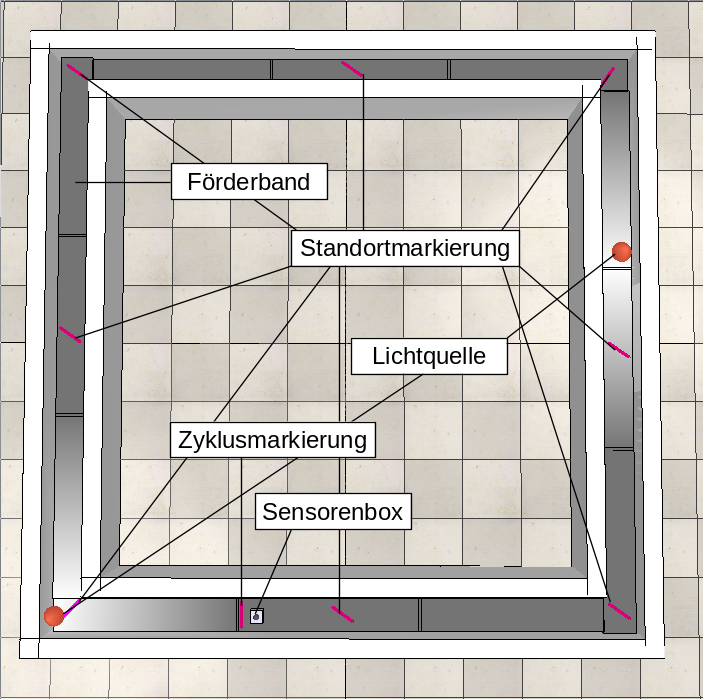
\includegraphics[width=\linewidth]{images/simple_square_labeled.png}
    \caption{Modell der Route \glqq simple\_square\grqq\ in CoppeliaSim mit Beschriftungen.}
    \label{fig:simple_square_labeled}
\end{figure}
\newline
\newline
Neben \glqq simple\_square \grqq\ gibt es noch drei weitere Routen (siehe Abbildungen \ref{fig:long_rectangle}, \ref{fig:rectangle_with_ramp} und \ref{fig:many_corners}).
Die Route \glqq long\_rectangle \grqq\ weist lange Pfade mit wenig Änderungen auf.
Die Route \glqq rectangle\_with\_ramp \grqq\ besitzt zusätzlich zwei Rampen, wodurch Höhenunterschiede simuliert werden.
Die Route \glqq many\_corners \grqq\ ist sehr komplex und hat viele verschiedene Standorte.
Die Förderbänder können verschiedene Geschwindigkeiten haben mit sowohl abrupten Übergangen, als auch fließenden Übergängen zueinander.
\newline
\newline
Je nach Enkodierungsart (siehe Kapitel \ref{sec:model_location_encoding}) müssen die Knoten und Kanten, dieses zyklischen Graphen, als Standorte enkodiert werden.
Als Knoten wird die Menge der Datensätze bezeichnet, die sich in einem Umkreis des ersten Datensatzes befinden, der mit einem Standort beschriftet ist,
d. h. Datensätze mit der gleichen Standortbeschriftung, die sich nicht im Umkreis des initialen Datensatzes befinden, gelten nicht als dieser Standort.
Die Knoten werden mit dem Wert der Standortbeschriftung beschriftet.
Die übrigen Datensätze werden entweder als unbekannten Standort beschriftet oder erhalten einen diskreten Standortwert, der die Beziehung der Kante zwischen zwei Knoten enkodiert.

\section{Künstlichen Sensordaten}
\begin{itemize}
    \item Motivation: Warum ist das nötig?
\end{itemize}

\subsection{Magnetfeld}
\begin{itemize}
    \item Welchen Sensor spiegelt das wieder?
    \item Wie funktioniert das Modell?
    \item Was und Wie wurden Daten ergänzt?
\end{itemize}

\subsection{Temperatur}
\begin{itemize}
    \item Welchen Sensor spiegelt das wieder?
    \item Wie funktioniert das Modell?
    \item Was und Wie wurden Daten ergänzt?
\end{itemize}

\subsection{Lautstärke}
\begin{itemize}
    \item Welchen Sensor spiegelt das wieder?
    \item Wie funktioniert das Modell?
    \item Was und Wie wurden Daten ergänzt?
\end{itemize}

\subsection{WLAN Zugangspunkte}
\begin{itemize}
    \item Welchen Sensor spiegelt das wieder?
    \item Wie funktioniert das Modell?
    \item Was und Wie wurden Daten ergänzt?
\end{itemize}

\section{Simulation von Interrupts}
\begin{itemize}
    \item Motivation => Energieverbrauch, Spiegelung der echten Datenaufnahme, Reduzierung der Trainingsdaten
    \item Wie funktioniert ist?
    \item Wie und Wann bei der Datenverarbeitung wird es gemacht?
    \item So wird bei einer Idle Box auch kein Interrupt erzeugt. (Sneaky Beispiel)
    \item Vorteile bei der Trainingszeit, da weniger Trainingsdaten
    \item Wie gut repräsentiert ist jeder Standort danach? => Graph vorher vs. nachher mit training sampling rate
    \item => Problem: Locations können einfach verpasst werden => Sampling rate?
    \item => Damit alle locations ausreichend in den Trainingsdaten repräsentiert sind, wird eine training sampling rate eingeführt
\end{itemize}

\section{Feature-Extrahierung}
\begin{itemize}
    \item Datenfenster: Realzeit vs. Diskret mittels Wakeups => Es werden immer die letzten 3 Behalten über die die Werte geglättet werden
    \item Relevanz von Zeit => Interrupts, Zeit als Feature, Feature können Zeit Abhängig und Unabhängig sein
    \item Welche Feature werden genutzt? => Abhängig von Feature Importance und wie günstig zu berechnen
    \item Wie werden diese extrahiert?
    \item Welchen Mehrwert verschaffen diese Features?
    \item Welchen Einfluss haben Sie im Hinblick auf Ressourcenbedarf(?), Klassifizierungsgenauigkeit(?), Fehlertoleranz(?)
    \item Rede über Feature Importance, insb. über Permutation Importance => Wie nützlich ist ein Sensor?
    \item Diskrete Distinct Location wird außerhalb verarbeitet => Modell verändern, dass die prev loc in Feature Processing step mit rein geht?
    \item Previous Location, Prev. Distinct Location vs. exponentiell abfallene letzte Orte diskutieren
\end{itemize}

\section{Fehlerhafte/Anomalie Daten}
\label{sec:data_anomalie}
\begin{itemize}
    \item Warum und Wieso?
    \item Welche Fehlerdaten werden eingebaut, was ist deren Begründung?
    \item Was ist eine Anomaly?
    \item Welche Anomalydaten wurden eingebaut?
    \item Welche Features werden zur Anomalierkennung extrahiert? Wie werden sie extrahiert? Wie funktioniert das in der Praxis?
    \item window deviation zu no anamoly data vs normal deviation zum avg
\end{itemize}

\section{Aufteilung der Daten}
\begin{itemize}
    \item Kurz und knapp wie und warum werden die Daten aufgeteilt. => Zyklen
    \item Sollten Trainingsdaten um synthetische Daten ergänzt werden?
    \begin{itemize}
        \item Fault Daten, um das Modell Robuster zu machen
        \item Synthetische Routen => Was ist das? Wie werden sie erzeugt?
    \end{itemize}
    \item Wie viele Trainingsdaten werden benötigt?
    \begin{itemize}
        \item Um KNN zu trainieren?
        \item Um Entscheidungsbaum zu trainieren?
        \item Ggf. Unterschiede klären
        \item (Gehört das schon in eine Evaluation, oder ist das hier okay?)
    \end{itemize}
\end{itemize}
\chapter{Evaluation}
In der Evaluation werden drei Aspekte betrachtet: Klassifizierungsgenauigkeit, Robustheit und Ressourcennutzung.
Bei der Klassifizierungsgenauigkeit wird einerseits die Standortbestimmung und andererseits die Anomalieerkennung evaluiert.
Dabei wird sowohl auf verschiedene Größen von FFNNs und Entscheidungswälder eingegangen,
als auch auf verschieden viele zu unterscheidende Standorte.
\newline
\newline
Bei der Robustheit wird auf den Fehler des besten FFNNs und Entscheidungswaldes bei verschiedenen Fehlerszenarien eingegangen.
Diese bestehen aus fehlerhaften Sensordaten durch Rauschen oder ausgefallenen Sensoren und Routen mit permutierten Teilstücken.
\newline
\newline
Bei der Ressourcennutzung wird auf die Programmgröße und die Ausführungszeit der besten ML-Modelle eingegangen.
Außerdem wird der Energieverbrauch für verschiedene Szenarien eingeschätzt.
\newline
\newline
Unterschieden werden zwei Varianten der Testmengen.
Diese unterscheiden sich in der Art, wie die Features für den vorherigen Standort bestimmt werden.
In der ersten Variante sind alle vorherigen Standorte korrekt.
In der zweiten Variante ist der erste vorherige Standort als \textit{unbekannt} beschriftet und alle folgenden vorherigen Standorte werden iterativ durch das ML-Modell bestimmt,
d.~h. in dieser Variante wird der propagierte Fehler durch die Rückwärtskante des ML-Modells betrachtet.
Metriken, die auf die zweite Variante der Testmenge angewendet werden sind mit \texttt{cont} markiert.
\newline
\newline
Die ML-Modelle wurden mit Trainingsdaten von den vier aufgenommen Routen trainiert.
Sie teilen ein relatives Koordinatensystem, in dem die künstlichen Interferenzquellen für die ergänzten Sensoren liegen.
Das heißt, ein Training mit mehreren Routen kann als eine sehr komplexe Route mit überlappenden Pfaden betrachtet werden,
da diese Routen technisch gesehen übereinander liegen.

\section{Metriken}
In dieser Arbeit werden verschiedene Metriken zur Ermittlung der Klassifizierungsgenauigkeit ermittelt.
Zunächst die übliche Klassifizierungsgenauigkeit (\ref{formular:simple_accuracy}), in der die Anzahl der korrekt klassifizierten Standorte mit der Gesamtanzahl verglichen werden.
\begin{align}
    \label{formular:simple_accuracy}
    P(A) := \frac{\text{Anzahl korrekter Klassifizierungen}}{\text{Gesamtanzahl}}
\end{align}
Die zweite Metrik (\ref{formular:accuracy_metrik2}) betrachtet die Klassifizierungsgenauigkeit unter Tolerierung, dass ein Standort
fünf bzw. zehn Klassifizierungen kontinuierlich zu früh oder zu spät verlassen wurde,
d.~h. Fehlklassifizierungen werden vernachlässigt, wenn kontinuierlich der letzte korrekte Standort bzw. der nächste korrekte
Standort klassifiziert wird mit einer Gesamttoleranz von fünf bzw. zehn Klassifizierungen.
\begin{flalign}
    \label{formular:accuracy_metrik2}
    &\epsilon \in \{5, 10\} \nonumber\\
    &L := \text{Menge von dem ML-Modell klassifizierten Standorte.} \nonumber\\
    &K := \text{Menge von den wirklichen Standorten.} \nonumber\\
    &\Phi(i) := \text{Index von dem nächsten Standort.} \nonumber\\
    &\Psi(i) := \text{Index von dem vorherigen Standort.} \nonumber\\
    &\Omega(i) := \Phi(i)-i\leq\epsilon\wedge\hspace{-0.3cm} \bigwedge\limits_{i\leq q \leq \min(\#K, \Phi(i))}\hspace{-0.3cm} L_q=K_{\Phi(i)} \nonumber\\
    &\Theta(i) := i-\Psi(i)\leq\epsilon\wedge\hspace{-0.3cm} \bigwedge\limits_{\max(0, \Psi(i))\leq q \leq i}\hspace{-0.3cm} L_q=K_{\Psi(i)} \nonumber\\
    &P(B) := \frac{\#\{L_i | L_i=K_i \vee \Omega(i) \vee \Theta(i)\text{ für } i\in\{0, 1, ..., \#L - 1\}\}}{\#K}
\end{flalign}
Zuletzt zwei Metriken bei denen die Klassifizierungsgenauigkeit bestimmt wird, unter der Bedingung, dass der vorherige
Standort korrekt (\ref{formular:accuracy_previous_was_correct}) bzw. falsch (\ref{formular:accuracy_previous_was_wrong}) war.
\begin{align}
    \label{formular:accuracy_previous_was_correct}
    P(C) := \frac{\text{Anzahl korrekter Klassifizierungen, wenn vorheriger Standort korrekt war}}{\text{Alle Klassifizierungen, wenn vorheriger Standort korrekt war}}
\end{align}
\begin{align}
    \label{formular:accuracy_previous_was_wrong}
    P(D) := \frac{\text{Anzahl korrekter Klassifizierungen, wenn vorheriger Standort falsch war}}{\text{Alle Klassifizierungen, wenn vorheriger Standort falsch war}}
\end{align}
\section{Klassifizierungsgenauigkeit der Standorte}
Die Klassifizierungsgenauigkeit der ML-Modelle zur Standorterkennung wurde mit verschiedenen Konfigurationen über komplexer werdende Datenmengen evaluiert.
In Kapitel \ref{sec:model_dt} und Kapitel \ref{sec:model_ffnn} werden die einzelnen Konfigurationen der ML-Modelle beschrieben.
Die Komplexität wird über die Anzahl der Standorte definiert.
Um die Anzahl der Standorte zu erhöhen, wurden die Datenmengen um weitere Routen erweitert.
Dies impliziert aber, dass die Testmengen nicht vergleichbar sind unter den Standortanzahlen, da mit jeder Route auch die Testmenge erweitert wird.
Die berechneten Klassifizierungswahrscheinlichkeiten sind jeweils der Durchschnitt der Klassifizierungswahrscheinlichkeiten aller Routen in der Testmenge.
\newline
\newline
Außerdem unterscheiden sich die Enkodierungsansätze je nach Standortanzahl.
Für die Standortanzahlen 9, 17, 25 und 52 wurde der Enkodierungsansatz verwendet, bei denen nur die Knoten und ein zusätzlicher unbekannter Standort betrachtet wird.
Für die Standortanzahlen 16, 32, 48 und 102 wurde der Enkodierungsansatz verwendet, bei denen Knoten und Kanten betrachtet werden.
Ein besserer Ansatz, um Daten mit beliebiger Komplexität zu generieren wird in Kapitel \ref{chapter:discussion} diskutiert.
\newline
\newline
Zunächst wird die Klassifizierungsgenauigkeit $P(A)$ im Vergleich zu Mians Ergebnissen betrachtet.
Mian konnte mit einem WFFNN bei einer Route mit drei Pfaden und 14 Standorten eine Klassifizierungsgenauigkeit von 94,1\% erreichen \cite{naveedThesis}.
Abbildung \ref{fig:best_dt_acc_vs_knn_acc_vs_cont} vergleicht die Klassifizierungsgenauigkeiten der
Entscheidungsbaum basierten Klassifizierer und FFNN über verschiedene Standortkomplexitäten.
Dabei wurde stets die höchste Klassifizierungsgenauigkeiten aller evaluierten Konfigurationen ausgewählt.
Gezeigt werden sowohl die Klassifizierungsgenauigkeiten auf die Testmengen die korrekt beschriftet sind und die, die von den ML-Modellen beschriftet sind.
\begin{figure}[h!]
    \centering
    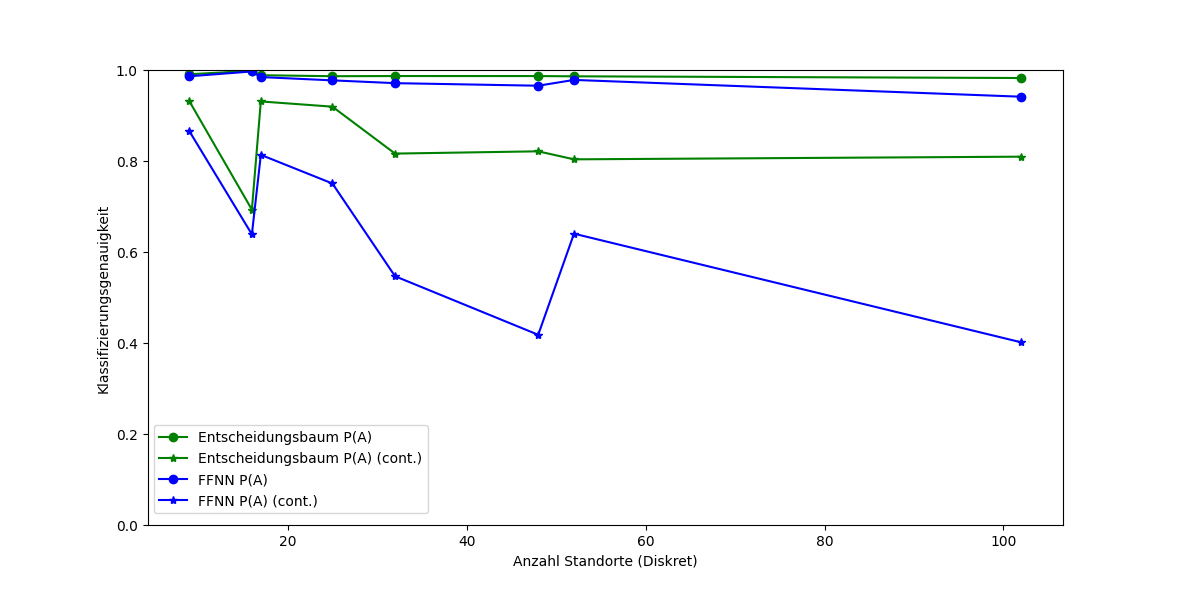
\includegraphics[width=\linewidth]{images/best_dt_vs_knn_acc_vs_acc_cont.png}
    \caption{Die besten Klassifizierungsgenauigkeiten aller evaluierten Konfigurationen der ML-Modelle über alle Standortkomplexitäten.}
    \label{fig:best_dt_acc_vs_knn_acc_vs_cont}
\end{figure}
\newline
\newline
Mian hat in seiner Evaluation die Klassifizierungsgenauigkeit $P(A)$ betrachtet.
Die in dieser Arbeit evaluierten Standortkomplexität, die Mians Evaluation am nächsten kommt ist 16.
Im Vergleich ist der beste Entscheidungsbaum basierte Klassifizierer mit einer Klassifizierungsgenauigkeit von 99,9\%, 5,8 Prozentpunkte besser
und das beste FFNN mit einer Klassifizierungsgenauigkeit von 99,79\%, 5,69 Prozentpunkte besser (Tabelle \ref{tab:predictions_by_acc}).
\newline
\newline
Dies betrachtet aber nicht den propagierten Fehler, der durch die Rekursion der ML-Modelle entsteht.
In Abbildung \ref{fig:best_dt_acc_vs_knn_acc_vs_cont} ist zu sehen, dass die Klassifizierungsgenauigkeit signifikant geringer ist bei allen Standortkomplexitäten.
Besonders mit der Standortkomplexität 16 ist die Klassifizierungsgenauigkeit signifikant geringer, wobei dies eine Artefakt der Enkodierungsmethode sein kann,
da bei der Standortkomplexität 17 immernoch Entscheidungsbaum basierte Klassifizierer mit einer Klassifizierungsgenauigkeit von 95,86\% gefunden wurden (Tabelle \ref{tab:predictions_by_acc_cont}).
Die FFNNS hingegen erreichen lediglich maximal 88,1\% bei dieser Standortkomplexität.
\newline
\newline
Aus Tabelle \ref{tab:predictions_by_acc_10_cont} können die Klassifizierungsgenauigkeiten $P(B=10)$ entnommen werden.
Der Entscheidungsbaum basierte Klassifizierer skaliert dabei sehr gut mit der steigenden Standortkomplexität.
Aber einer Standortkomplexität von 32 wird konnte aber nurnoch eine Klassifizierungsgenauigkeit von 91,35\% erreicht werden, die bis auf 87,87\% bei 102 Standorten fällt.
Als beste maximale Baumhöhe hat sich 16 herausgestellt, wobei 32 und 64 marginal schlechtere Ergebnisse produzierten.
Eine maximale Baumhöhe von 8 war nicht ausreichend und hat sich hat deutlich schlechtere Ergebnisse erzielt.
Bei gleicher Waldgröße haben die maximalen Baumhöhen und 32 und 64 equivalente Ergebnisse produziert.
Die verschiedenen Waldgrößen unterscheiden sich nicht stark.
Eine Waldgröße von 8 hat nur marginal schlechtere Ergenisse bei 102 Standorten erzielt, als die Waldgrößen 16, 32 und 64.
Aus diesem Grund ist eine Waldgröße von 8 ausreichend, oder könnte womöglich immernoch reduziert werden.
\newline
\newline
Die evaluierten FFNNs skalieren deutlich schlechter als die Entscheidungsbaum basierten Klassifizierer mit steigender Standortkomplexität.
Besonders die FFNNs der Standortkomplexitäten, die das Enkodierungsverfahren der Kanten und Knoten nutzte,
konnten signifikant schlechtere Klassifizierungsergebnisse erzielen als die FFNNs die das andere Enkodierungsverfahren nutzten.
Aus den Daten ist nicht zu schließen, wie sich die Anzahl der Schichten und Neuronen pro Schicht auf die Klassifizierungsgenauigkeit auswirkt.
Für geringe Standortkomplexitäten haben vermehrt kleine FFNNs besser abgeschnitten und für große Standortkomplexitäten vermehrt große FFNNs.
\begin{table}[h!]
    \hspace{-1.5cm}
    \begin{tabular}{ | c | c | c | c | c | c | c | c | c | c | }
        \hline
        \multicolumn{2}{ | l |}{$P(B=10)_{\text{cont}}$ über Standorte} & 9 & 16 & 17 & 25 & 32 & 48 & 52 & 102 \\\hline
        \multicolumn{10}{| l |}{\textbf{Entscheidungswälder}}\\\hline
        Waldgröße & Max. Baumgröße & \multicolumn{8}{ c |}{}\\\hline
        16 & 8 & 99.88 & 81.69\% & 99.50\% & 94.21\% & 82.88\% & 88.40\% & 85.72\% & 79.01\% \\\hline
        16 & 16 & 99.78 & 77.30\% & 99.73\% & 93.40\% & 91.35\% & 92.86\% & 89.86\% & 89.10\% \\\hline
        16 & 32 & 99.78 & 77.00\% & 99.83\% & 98.31\% & 86.55\% & 92.60\% & 90.66\% & 85.69\% \\\hline
        16 & 64 & 99.78 & 77.00\% & 99.83\% & 98.31\% & 86.55\% & 92.60\% & 90.66\% & 85.69\% \\\hline
        8 & 32 & 98.92 & 92.79\% & 99.66\% & 98.10\% & 90.27\% & 91.45\% & 89.46\% & 85.11\% \\\hline
        16 & 32 & 99.78 & 77.00\% & 99.83\% & 98.31\% & 86.55\% & 92.60\% & 90.66\% & 85.69\% \\\hline
        32 & 32 & 99.79 & 78.06\% & 99.63\% & 97.52\% & 88.83\% & 93.33\% & 89.20\% & 86.92\% \\\hline
        64 & 32 & 99.69 & 84.66\% & 99.82\% & 97.62\% & 89.65\% & 93.31\% & 86.15\% & 87.87\% \\\hline
        32 & 64 & 99.79 & 78.06\% & 99.63\% & 97.52\% & 88.83\% & 93.33\% & 89.20\% & 86.92\% \\\hline
        \multicolumn{10}{| l |}{\textbf{Feed Forward neuronale Netzwerke}}\\\hline
        \#Schichten & \#Neuronen & \multicolumn{8}{ c |}{}\\\hline
        1 & 16 & 99.65 & 76.69\% & 93.25\% & 83.76\% & 45.93\% & 65.16\% & 76.85\% & 42.39\% \\\hline
        1 & 32 & 99.77 & 77.04\% & 93.47\% & 84.28\% & 63.63\% & 64.21\% & 76.40\% & 44.73\% \\\hline
        1 & 64 & 99.69 & 68.52\% & 95.35\% & 88.93\% & 50.44\% & 83.60\% & 80.52\% & 33.87\% \\\hline
        1 & 128 & 99.10 & 75.39\% & 92.96\% & 91.02\% & 52.27\% & 55.62\% & 82.18\% & 42.56\% \\\hline
        2 & 32 & 98.59 & 63.99\% & 96.98\% & 87.72\% & 68.52\% & 73.21\% & 79.07\% & 35.48\% \\\hline
        4 & 32 & 99.61 & 71.53\% & 93.63\% & 93.19\% & 49.47\% & 52.64\% & 82.16\% & 38.66\% \\\hline
        8 & 32 & 92.74 & 62.31\% & 86.52\% & 86.57\% & 36.36\% & 71.92\% & 75.98\% & 51.15\% \\\hline
        4 & 64 & 99.06 & 67.74\% & 93.76\% & 94.15\% & 54.47\% & 47.75\% & 82.08\% & 47.55\% \\\hline
    \end{tabular}
    \caption{Metrik $P(B=10)_{\text{cont}}$ über Standorte und verschiedenen Konfigurationen der ML-Modelle.}
    \label{tab:predictions_by_acc_10_cont}
\end{table}
\section{Klassifizierungsgenauigkeit der Anomalien}
\label{sec:eval_anomalieerkennung}
Bei der Anomalieerkennung werden Entscheidungswälder und FFNNs mit den besten ML-Modellen zur Standorterkennung trainiert und mit den drei Baseline-Modellen verglichen.
Tabelle \ref{tab:anomaly_detection_prediction_accuracy} zeigt die Klassifizierungsgenauigkeiten über die verschiedenen Standortkomplexitäten,
wobei die Klassifizierungsgenauigkeit $P(A)$ nochmal genauer aufgeschlüsselt ist in den Anteil der korrekten Klassifizierungen, wenn eine bzw. keine Anomalie vorlag.
Die trainierten FFNNs geben stets aus, dass keine Anomalie vorliegt.
Es ist unklar, warum die FFNNs sich so verhalten.
\begin{table}[h!]
    \hspace{-1cm}
    \begin{tabular}{ | l | c | c | c | c | c | c | c | c | }
        \hline
        Standorte & 9 & 16 & 17 & 25 & 32 & 48 & 52 & 102 \\\hline
        \multicolumn{9}{ | l |}{$P(A)$}\\\hline
        Entscheidungswald & 82,59\% & 81,19\% & 87,14\% & 84,91\% & 79,06\% & 83,47\% & 81,93\% & 76,00\% \\\hline
        FFNN & 77,88\% & 77,88\% & 77,88\% & 77,88\% & 77,88\% & 77,88\% & 77,88\% & 77,88\% \\\hline
        Topologie (DT) & 84,77\% & 30,57\% & 83,51\% & 79,76\% & 28,63\% & 24,97\% & 80,55\% & 29,47\% \\\hline
        Topologie (KNN) & 86,10\% & 52,17\% & 77,72\% & 79,30\% & 45,06\% & 41,92\% & 74,77\% & 43,55\% \\\hline
        \multicolumn{9}{ | l |}{Anteil korrekt klassifiziert, indem Anomalie vorlag}\\\hline
        Entscheidungswald & 34,86\% & 35,52\% & 52,58\% & 50,92\% & 32,21\% & 50,64\% & 23,21\% & 1,92\% \\\hline
        FFNN & 0,00\% & 0,00\% & 0,00\% & 0,00\% & 0,00\% & 0,00\% & 0,00\% & 0,00\% \\\hline
        \multicolumn{9}{ | l |}{Anteil korrekt klassifiziert, indem keine Anomalie vorlag}\\\hline
        Entscheidungswald & 96,14\% & 94,41\% & 97,05\% & 95,83\% & 92,48\% & 93,13\% & 98,96\% & 97,18\% \\\hline
        FFNN & 100,00\% & 100,00\% & 100,00\% & 100,00\% & 100,00\% & 100,00\% & 100,00\% & 100,00\% \\\hline
    \end{tabular}
    \caption{$P(A)$ über Standorte und Modelle zur Anomalieerkennung.}
    \label{tab:anomaly_detection_prediction_accuracy}
\end{table}
\newpage
Die Entscheidungswälder hingegen eignen sich besser für den Anomalieerkennungszweck.
Es werden zwischen 1,92\% und 52,58\% der Anomalien erkannt und zwischen 1,04\% und 7,52\% falsch als Anomalien erkannt.
Die Klassifizierungsgenauigkeit des Entscheidungswaldes zur Anomalieerkennung ist abhängig von der Klassifizierungsgenauigkeit zur Standorterkennung
und von der Standortkomplexität.
Je besser das Standorterkennungsmodell und je höher die Standortkomplexität, desto höher ist die Anomalieerkennungsrate.
Aus diesem Grund ist die Klassifizierungsgenauigkeit bei den Standortkomplexitäten, die mit der Kodierungsmethode mit Kanten und Knoten zusammenhängen,
geringer, als bei der Kodierungsmethode, bei der nur die Knoten kodiert werden.
\newline
\newline
Abbildung \ref{fig:true_vs_predicted_anomaly} zeigt einen Auscchnitt der Anomalietestmenge, worauf der Entscheidungswald der Standortkomplexität 17 angewendet wurde.
Die Anomalie wird nicht kontinuierlich erkannt und es werden auch fälschlicherweise Standorte als Anomalien klassifiziert.
Allerdings treten falsch-positive Ergebnisse nur vereinzelt auf, wohingegen bei einer Anomalie, sehr häufig eine Anomalie erkannt wird.
Die falsch-positiven Ergebnisse können somit durch Ausnutzen dieser Fluktuationen vermieden werden,
indem beispielweise ein Schwellenwert an Ausschlägen in einer bestimmten Zeit eingeführt wird.
\begin{figure}[h!]
    \centering
    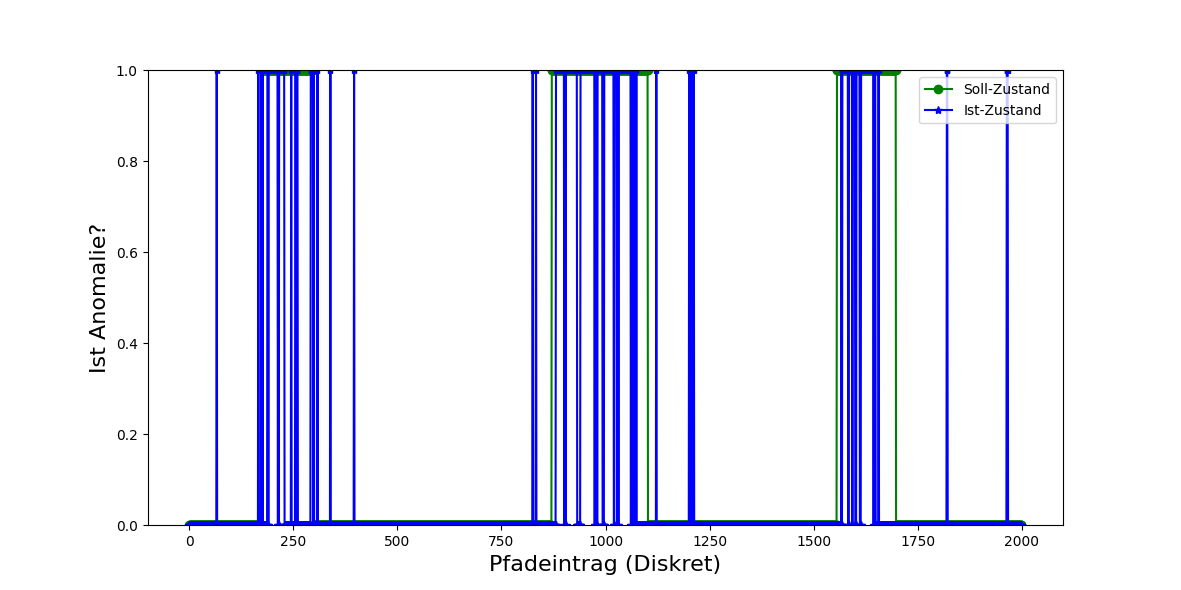
\includegraphics[width=\linewidth]{images/anomaly_true_vs_predicted.png}
    \caption{Ausschnitt der Klassifizierungsergebnisse auf der Anomalietestmenge mit dem Entscheidungswald der Standortkomplexität 17. }
    \label{fig:true_vs_predicted_anomaly}
\end{figure}
\section{Signifikanz der Features}
Die Signifikanz der Features wird über die Permutationswichtigkeit bestimmt.
Die Permutationswichtigkeit ist der Fehler, der durch das permutieren eines Features in der Testmenge entsteht, im Vergleich zu der ursprünglichen Testmenge.
Je größer der Fehler, desto wichtiger das Feature.
\newline
\newline
Abbildungen \ref{fig:feature_significance_dt} und \ref{fig:feature_significance_knn} zeigen die Permutationswichtigkeit eines Entscheidungswaldes und FFNN.
Die Permutationswichtigkeit von einzelnen Entscheidungswäldern bzw. FFNNs unterscheidet sich nicht stark.
Beide ML-Modelle weisen den vorherigen Standorten eine hohe Signifikanz zu.
Die Klassifizierunggenauigkeiten in Tabelle \ref{tab:predictions_by_acc_pic_cont} bestätigen diese Abhängigkeit.
Demnach ist die Wahrscheinlichkeit sehr gering, dass der Standort korrekt klassifiziert wird, wenn der vorherige Standort inkorrekt war.
\begin{figure}[h!]
    \centering
    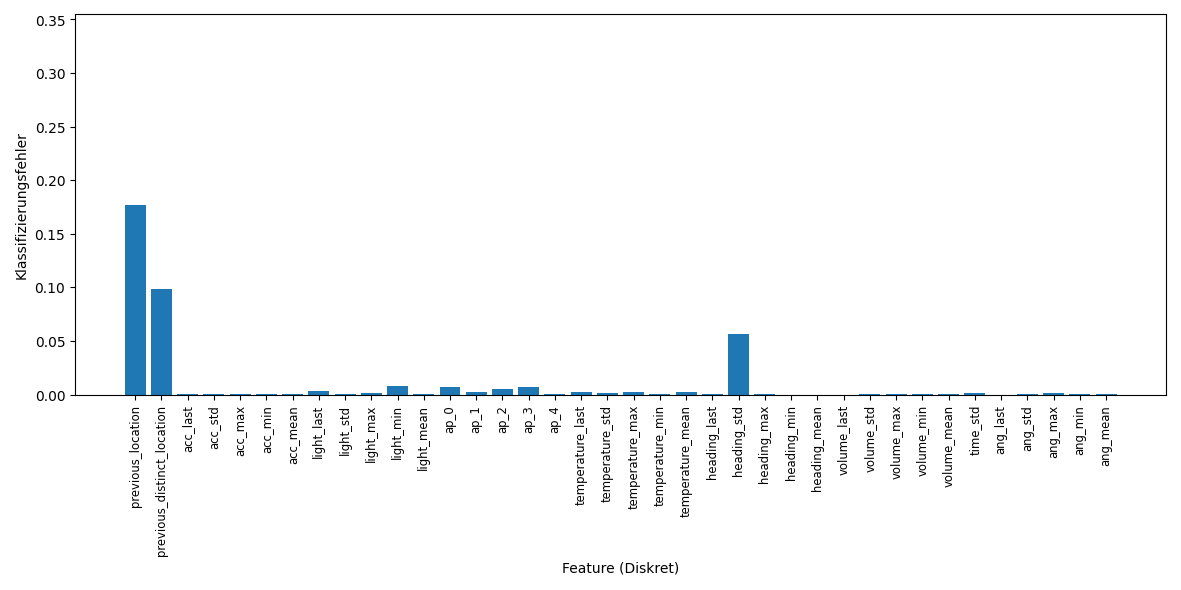
\includegraphics[width=\linewidth]{images/evaluation_feature_importance_dt_pi.png}
    \caption{Permutationswichtigkeit der Features eines Entscheidungswaldes.}
    \label{fig:feature_significance_dt}
\end{figure}
\begin{figure}[h!]
    \centering
    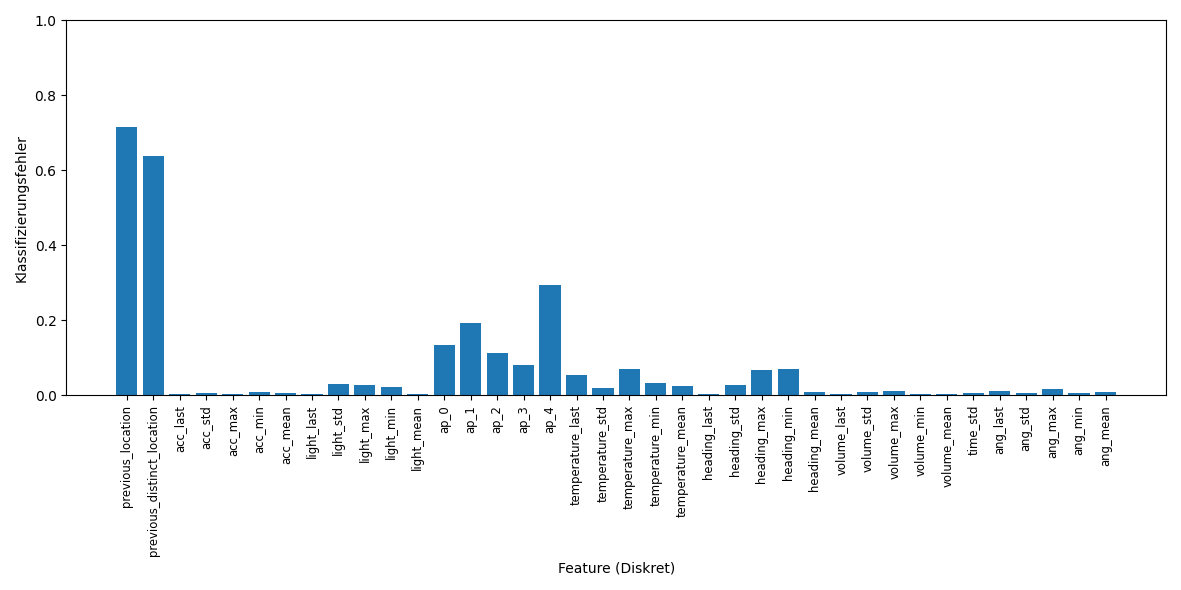
\includegraphics[width=\linewidth]{images/evaluation_feature_importance_knn_pi.png}
    \caption{Permutationswichtigkeit der Features eines FFNN.}
    \label{fig:feature_significance_knn}
\end{figure}
\newline
\newline
Für die Entscheidungswälder sind alle Features, bis auf die vorherige Position und die Standardabweichung in der Ausrichtung zum Magnetfeld unwichtig.
Die FFNNs hingegen bedienen sich außerdem Features von dem Temperatursensor, dem Lichtsensor und vor allem der Detektierung von WLAN-Zugangspunkten.
Allerdings sind FFNNs deutlich abhängiger von dem vorherigen Standort als Entscheidungswälder.
\newline
\newline
Durch diese Abhängigkeit ist keine hohe Robustheit zu erwarten der ML-Modelle zu erwarten.
Diese Abhängigkeit ließe sich Eliminieren, indem ohne die Rückwärtskante trainiert wird.
Dies simplifiziert den Trainingsprozess, wodurch die ML-Modelle schneller zu trainieren sind.
Tabelle \ref{tab:predictions_wo_feedback_edge_by_acc} zeigt, dass diese ML-Modelle vergleichbare Klassifizierungsgenauigkeiten erzielen.
Insbesondere FFNNs erzielen deutlich bessere Klassfizierungsgenauigkeiten, erzielen aber dennoch schlechtere Ergebnisse als die Entscheidungswälder.
Hier ist die Metrik $P(A)$ mit der Metrik $P(A)_{\text{cont}}$ vergleichbar, da der propagierte Fehler durch die Eliminierung der Rückwärtskante nicht mehr existiert.
\newline
\newline
Abbildungen \ref{fig:feature_significance_dt_wo_fe} und \ref{fig:feature_significance_knn_wo_fe} zeigen die Permutationswichtigkeit der ML-Modelle ohne Rückwärtskante.
Beide ML-Modelle gewichten Features aus anderen Sensorwerten deutlich mehr, im Vergleich zu den ML-Modellen mit Rückwärtskante.
Die Entscheidungswälder gewichten dennoch nur die Standardabweichung der Ausrichtung zum Magnetfeld, due Detektierung der WLAN-Zugangspunkte und das Minimum des Lichtsensors stark.
Die anderen Features sind im Vergleich deutlich unwichtiger.
Das FFNN hingegen nutzt alle Features, wobei Features aus dem Accelerometer und Gyroskop unwichtiger sind.
\begin{figure}[h!]
    \centering
    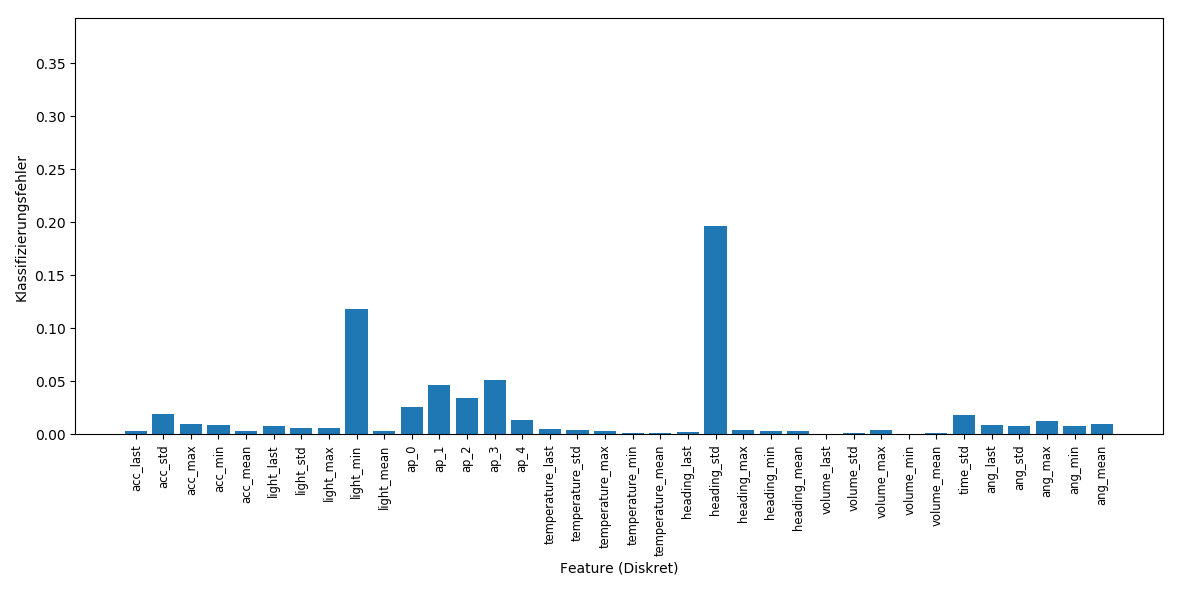
\includegraphics[width=\linewidth]{images/fi_wo_fe_dt.png}
    \caption{Permutationswichtigkeit der Features eines Entscheidungswaldes ohne Rückwärtskante.}
    \label{fig:feature_significance_dt_wo_fe}
\end{figure}
\begin{figure}[h!]
    \centering
    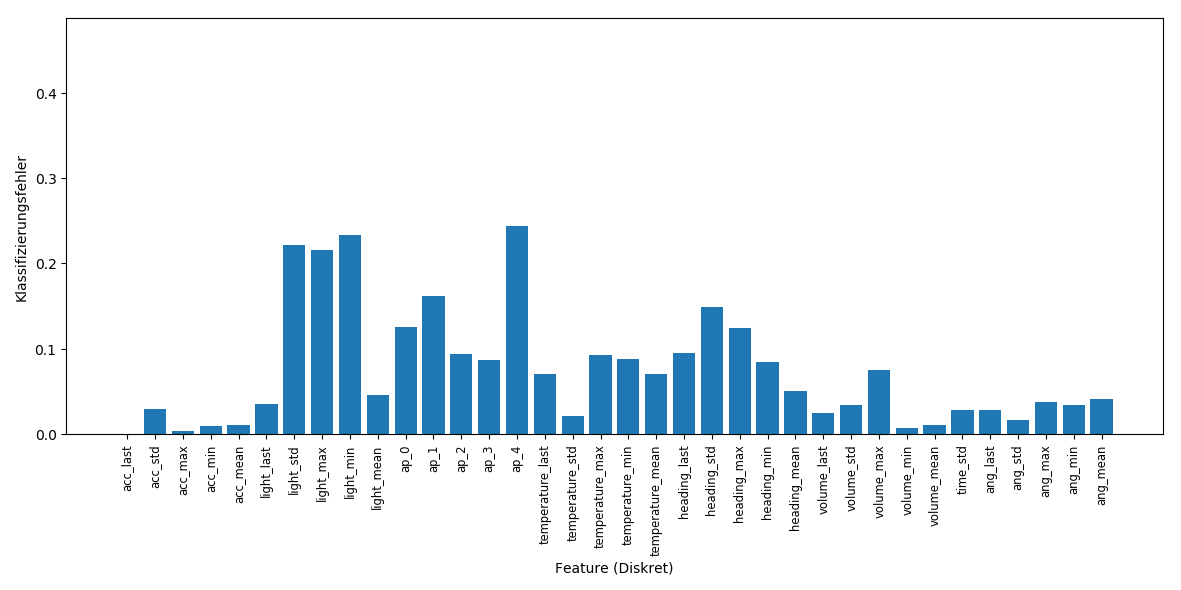
\includegraphics[width=\linewidth]{images/fi_wo_fe_knn.png}
    \caption{Permutationswichtigkeit der Features eines FFNN ohne Rückwärtskante.}
    \label{fig:feature_significance_knn_wo_fe}
\end{figure}
\section{Fehlertoleranz}
Bei der Fehlertoleranz wird die Fähigkeit der ML-Modelle untersucht, trotz fehlerhafter Sensordaten Standorte zu erkennen.
Dafür wurden für jeden Sensor modifizierte Testmengen erstellt.
Die erste Testmenge fügt ein Rauschen von 5\% hinzu und die zweite Testmenge simuliert den Ausfall des Sensors, indem alle Sensorwerte genullt werden.
Zudem wurde untersucht, was passiert wenn die Sensorenbox nicht dem trainierten Pfad folgt, indem die Testmenge permutiert wurde.
Damit Entscheidungswald und FFNN fair verglichen werden können, werden die besten ML-Modelle der Standortkomplexität 9 verwendet.
\newline
\newline
Tabelle \ref{tab:robustness} zeigt die Differenz der Klassifizierungsgenauigkeiten $P(A)_{\text{cont}}$ und $P(A)$ von den modifizierten Testmengen zur originalen Testmenge.
Die Testmengen mit einem Rauschen von 5\% wurde ausgelassen, da es keine Auswirkung auf die Klassifizierungsgenauigkeit hatte.
Vermutlich ist 5\% Rauschen zu wenig, um einen Einfluss auszuüben.
\begin{table}[h!]
    \hspace{-1.25cm}
    \begin{tabular}{ | l | c | c | c | c | }
        \hline
        Testmenge & Entscheidungswald & FFNN & Entscheidungswald & FNNN \\\hline
        & \multicolumn{2}{ c }{mit Rückwärtskante} & \multicolumn{2}{| c |}{ohne Rückwärtskante} \\\hline
        Licht & 4.46\%-Pkt. & 4.65\%-Pkt. & 5.28\%-Pkt. & 6.93\%-Pkt \\\hline
        Geräusch & 3.20\%-Pkt. & 5.00\%-Pkt. & 1.63\%-Pkt. & 5.11\%-Pkt. \\\hline
        Temperatur & 15.15\%-Pkt. & 6.60\%-Pkt. & 8.10\%-Pkt. & 13.50\%-Pkt. \\\hline
        Ausrichtung zum Magnetfeld & 3.32\%-Pkt. & 19.94\%-Pkt. & 2.51\%-Pkt. & 2.78\%-Pkt. \\\hline
        WLAN-Zugangspunkte & 2.60\%-Pkt. & 22.65\%-Pkt. & 3.74\%-Pkt. & 14.13\%-Pkt. \\\hline
        Accelerometer & 1.41\%-Pkt. & 9.52\%-Pkt. & 0.62\%-Pkt. & 1.33\%-Pkt. \\\hline
        Gyroskop & 8.52\%-Pkt. & 4.58\%-Pkt. & 0.91\%-Pkt. & 3.30\%-Pkt. \\\hline
        Permutierte Testmenge & 2.27\%-Pkt. & -0.13\%-Pkt. & 0.47\%-Pkt. & 0.93\%-Pkt. \\\hline
        \textbf{Durchschnitt} & \textbf{5,8\%-Pkt.} & \textbf{9,1\%-Pkt.} & \textbf{2,91\%-Pkt.} & \textbf{6,00\%-Pkt.} \\\hline
    \end{tabular}
    \caption{Fehler der modifizierten Testmengen zur originalen Testmenge.}
    \label{tab:robustness}
\end{table}
\newline
\newline
Die ML-Modelle mit und ohne Rückwärtskante sind robust gegenüber der Nullung der Features und gegenüber der permutierten Testmenge.
Aus der Menge stechen die Fehler durch die Nullung der Features des Temperatur- und Magnetfeldsensors sowie der WLAN-Zugangspunkte heraus.
Außerdem ist der Fehler durch die Nullung der Features des Accelerometers und Gyroskops bei den ML-Modellen mit Rückwärtskanten
deutlich größer als bei den ML-Modellen ohne Rückwärtskante.
\newline
\newline
Die Permutationswichtigkeit hat den Features des Temperatursensors eine geringere Wichtigkeit zugeordnet, als die Nullung es tut.
Dies ist dadurch begründet, dass die Sensordaten des Temperatursensors mit wenigen Ausnahmen sehr homogen sind.
Für den Temperatursensor wird eine Umgebungstemperatur simuliert, die sich nur verändert, wenn die Sensorenbox einer Wärmequelle näher kommt.
Für den größten Teil der Daten misst der Temperatursensor die Umgebungstemperatur, weswegen eine permutation keinen großen Fehler verursacht.
Die Nullung dieser Sensordaten hingegen deutet auf eine Wärmequelle hin, die die Umgebungstemperatur verringert.
Dieses Ereignis ist im Vergleich zu einer Erhöhung der Umgebungstemperatur selten, weswegen die Nullung einen großen Fehler verursacht.
Würde dieses Ereignis häufiger vorkommen, wäre der Fehler vermutlich geringer.
\newline
\newline
Das FFNN mit Rückwärtskante hat im Vergleich zu den anderen ML-Modellen einen deutlich größeren Fehler, wenn die Features des Magnetfeldsensors genullt werden.
Diese Anomalie ist entgegen den Erwartungen der Permutationswichtigkeit, insbesondere da die anderen ML-Modelle
höhere Permutationswichtigkeiten für die Features des Magnetfeldsensors erzeugt haben.
Es ist unklar, warum das FFNN, im Vergleich zu den anderen ML-Modellen, dem so anfällig ist.
\newline
\newline
Die FFNNs erzeugen einen großen Fehler, wenn die WLAN-Zugangspunkte genullt werden.
Dies stimmt mit den Ergebnissen der Permutationswichtigkeit überein.
Insgesamt bilden die Features der WLAN-Zugangspunkte 14,7\% aller Features, wobei die Werte bei der Eingabeschicht binär sind.
Vermutlich ist aus diesem Grund der Einfluss dieser Features beim FFNN im Vergleich zu den Entscheidungswäldern so groß.
\newline
\newline
Die Permutation der Testmenge hat nur einen geringen Fehler verursacht.
Dies war bei allen ML-Modellen zu erwarten, da das interne Datenfenster mit drei Einträgen sehr klein ist
und die Features der vorherigen Standorte bereits nach wenigen Klassifizierungen korrigiert werden.
Dementsprechend ist der Fehler bei den ML-Modellen ohne Rückwärtskante auch deutlich kleiner als bei den ML-Modellen mit Rückwärtskante.
\newpage
Im Durchschnitt sind die ML-Modelle ohne Rückwärtskante robuster als die ML-Modelle mit Rückwärtskante.
Die Entscheidungswälder sind robuster als die FFNNs.
Der beobachtete Fehler korreliert aber mit der Klassifizierungsgenauigkeit der ML-Modelle (Abbildung \ref{fig:best_dt_vs_knn_fb_vs_no_fb}).
Der Entscheidungswald mit Rückwärtskante, der marginal bessere Klassifizierungsgenauigkeiten erzielt hat, als das FFNN ohne Rückwärtskante,
hat einen marginal geringeren Fehler im Test erzielt.
\newline
\newline
Tabellen \ref{tab:predictions_by_acc_pic_cont} und \ref{tab:predictions_by_acc_pic_wo_fb} geben die Klassifizierungsgenauigkeit $P(C)_{\text{cont}}$ bzw. $P(C)$ an.
Diese geben die Wahrscheinlichkeit an, dass ein Standort korrekt klassifiziert wird, wenn der Standort zuvor falsch klassifiziert wurde.
Wie zu erwarten ist die Wahrscheinlichkeit bei den ML-Modellen ohne Rückwärtskante deutlich größer.
Bei einer Standortkomplexität von 9 Orten benötigt ein Entscheidungswald mit Rückwärtskante ca. 5,3 Klassifizierungen,
ein FFNN mit Rückwärtskante ca. 5,8 Klassifizierungen, ein Entscheidungswald ohne Rückwärtskante ca. 1,9 Klassifizierungen
und ein FFNN ohne Rückwärtskante ca. 2,2 Klassifizierungen.
Bei einer Standortkomplexität von 102 Orten werden 8,1-, 25-, 3,4- und 4,4 Klassifizierungen benötigt.
Dies bestätigt, dass die ML-Modelle ohne Rückwärtskante deutlich robuster sind als die mit Rückwärtskante.
\newline
\newline
Von Entscheidungswäldern ist zu erwarten, dass sie mit steigender Waldgröße robuster werden, da sich die Feature-Mengen der einzelnen Entscheidungsbäume unterscheiden.
Dies wird von den Klassifizierungsergebnissen teilweise gestützt, allerdings ist unklar, ob dies nicht nur mit der damit steigenden Klassifizierungsgenauigkeit zusammenhängt.
\newline
\newline
Im Vergleich zu Mian sind die ML-Modelle dieser Arbeit deutlich robuster.
Der Ausfall des Lichtsensors bei Mians Ansätzen hat einen Fehler von 88,15 Prozentpunkten verursacht \cite{naveedThesis},
wohingegen der Fehler des schlechtesten ML-Modells in dieser Arbeit gegenüber dem Ausfall des Lichtsensors nur 6,93 Prozentpunkten ist.
\newline
\newline
In dieser Arbeit haben sich Entscheidungswälder als robuster gegenüber Fehler herausgestellt als FFNNs.
Allerdings erzielen die Entscheidungswälder in dieser Arbeit auch insgesamt bessere Klassifizierungsergebnisse, weswegen dies zu erwarten ist.
Der durchschnittliche Fehler beider ML-Modelle ist vergleichbar, bei vergleichbarer Klassifizierungsgenauigkeit.
Zusätzlich hat sich die Untersuchung von modifizierten Testmengen mit gezielten Veränderungen als Ergänzung zur Permutationswichtigkeit bewiesen,
um die Wichtigkeit von einzelnen Features einzuschätzen.
\section{Benötigte Trainingsdaten}
Mit wachsender Standortkomplexität werden mehr Trainingsdaten benötigt.
Abbildung \ref{fig:required_training_data} zeigt die benötigten Trainingszyklen für Entscheidungswälder und FFNNs mit Rückwärtskante bis auf der Testmenge
eine Klassifizierungsgenauigkeit $P(A)$ von 97\% erreicht wurde.
Es wurde 97\% als Grenze gewählt, da 97,26\% die höchste Klassifizierungsgenauigkeit des FFNNs bei einer Standortkomplexität von 102 ist.
Die Trainingszyklen korrelieren mit der Anzahl der Trainingsdaten, da mit jedem Zyklus die Trainingsdaten ergänzt werden.
\begin{figure}[h!]
    \centering
    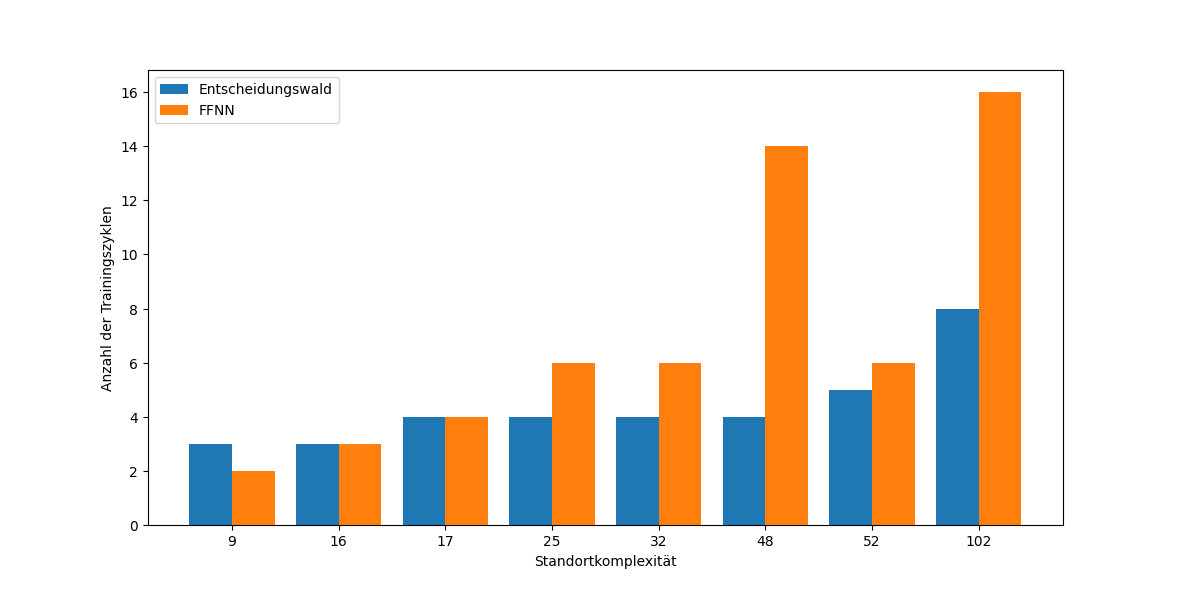
\includegraphics[width=\linewidth]{images/required_training_data.png}
    \caption{Anzahl der benötigten Trainingszyklen bis $P(A)=97\%$ auf der Testmenge erreicht wurde. }
    \label{fig:required_training_data}
\end{figure}
\newline
\newline
Die Entscheidungswälder benötigen weniger Trainingszyklen als FFNNs, um den Schwellenwert zu erreichen.
Je größer die Standortkomplexität, desto größer wird die Differenz der benötigten Trainingsdaten.
Die ML-Modelle ohne Rückwärtskante wurden nicht in Zyklen trainiert, weswegen keine Aussage über die benötigten Trainingsdaten getroffen wird.
\section{Programmspeicher}
Der Großteil des Programmspeichers wird für das ML-Modell benötigt.
Aus diesem Grund wird der Anteil des Programmspeichers $X$ in der Evaluation vernachlässigt,
der für die restlichen Funktionen und für die Feature-Extrahierung benötigt wird.
Zudem ist der benötigte Programmspeicher dieses Anteils konstant und skaliert nicht mit der Größe, wie die ML-Modelle.
\newline
\newline
Zur Estimierung des Programmspeichers der Entscheidungsbäume wird der hybride Ansatz mit einer Toleranz von $\epsilon=0$ angenommen,
d. h. es werden für eindeutige Ergebnisse diskrete Rückgaben zurückgegeben, anstatt der Wahrscheinlichkeitsverteilung.
Als Datentyp für die Vergleiche und allen Features wird angenommen, dass ein vier Byte Datentyp verwendet wird.
Für einen Vergleich werden fünf Instruktionen benötigt \cite{dymelThesis}.
Für eine Rückgabe werden zwischen zwei und $2(N+1)$ Instruktionen und zwischen 0 und $2N$ Parameter benötigt,
wobei $N$ die Anzahl der möglichen Standorte ist.
Die Größe einer Instruktion ist 4 Byte, da eine 32-Bit CPU angenommen wird.
Die Größe des zusammenfassenden Klassifizierers $Z$ wird vernachlässigt.
\newline
\newline
Für die FFNNs wird ebenfalls ein vier Byte Datentyp für die Biase und die Gewichte angenommen.
Die Größe des Algorithmus zur Ausführung des KNN ist unbekannt und wird als konstanter Wert $Y$ angenommen,
liegt aber, den Zahlen in Gieses Arbeit nach zu urteilen, zwischen 6 und 7 KB \cite{gieseThesis}.
\newline
\newline
Tabelle \ref{tab:predictions_by_loc_size} zeigt Estimierungen des benötigten Programmspeichers der verschiedenen Konfigurationen der ML-Modelle,
wobei die konstanten Anteile vernachlässigt werden.
Potentielle Optimierungen, z. B. durch den Compiler, wurden dabei nicht betrachtet,
sowie potentielle Optimierungen des FFNN, wie Giese sie vorgeschlagen hat \cite{gieseThesis}.
Giese hat mit dem CSC-MA-Bit Format die Programmgröße um 39\% reduzieren können.
Kompilierung mit der Optimierungsstufe \textit{O2} konnte experimentell generierten C-Code
eines Entscheidungswaldes um bis zu 21,3\% reduzieren.
\newline
\newline
Der benötigte Programmspeicher beider ML-Modelle skaliert mit der Anzahl der zu klassifizierenden Standorte, der Anzahl der Schichten bzw. Bäume
und der Anzahl der Neuronen pro Schicht bzw. der maximalen Baumhöhe.
Der von den Entscheidungswäldern benötigte Programmspeicher ist für fast alle Fälle zu viel
für die Limitierungen eines kleinen eingebetteten Systems.
Die FFNNs hingegen benötigen deutlich weniger Programmspeicher und könnten innerhalb der Limitierungen der kleinen eingebetten Systeme passen.
\newline
\newline
TODO: Braucht man mehr Neuronen/Hidden Layer mit steigender Ort Anzahl? (Hier oder bei ML-Modell FFNN)
\newline
TODO: Wie viel Speicherverbrauch spart man durch die Feature-Selection zusätzlich ein?
\begin{table}[h!]
    \hspace{-2cm}
    \begin{tabular}{ | c | c | c | c | c | c | c | c | c | c | }
        \hline
        \multicolumn{2}{ | l |}{Größe in KB über Standorte} & 9 & 16 & 17 & 25 & 32 & 48 & 52 & 102 \\\hline
        \multicolumn{10}{| l |}{\textbf{Entscheidungswälder}}\\\hline
        Waldgröße & Max. Baumgröße & \multicolumn{8}{ c |}{}\\\hline
        16 & 8 & 79.9 & 83.2 & 117.9 & 169.6 & 147.2 & 204.1 & 254.9 & 354.0 \\\hline
        16 & 16 & 192.2 & 199.0 & 277.4 & 512.7 & 371.1 & 750.4 & 914.4 & 1350.0 \\\hline
        16 & 32 & 185.7 & 197.6 & 287.2 & 550.2 & 394.5 & 875.6 & 1016.7 & 1582.3 \\\hline
        16 & 64 & 185.7 & 197.6 & 287.2 & 543.0 & 394.5 & 875.6 & 943.6 & 1582.3 \\\hline
        8 & 32 & 94.7 & 108.1 & 136.7 & 252.7 & 192.9 & 436.8 & 465.6 & 753.8 \\\hline
        16 & 32 & 185.7 & 197.6 & 287.2 & 550.2 & 394.5 & 875.6 & 1016.7 & 1582.3 \\\hline
        32 & 32 & 364.8 & 401.7 & 575.7 & 1055.9 & 803.9 & 1701.0 & 1962.6 & 3061.1 \\\hline
        64 & 32 & 776.1 & 842.8 & 1173.8 & 2132.7 & 1584.7 & 3455.2 & 3987.8 & 6327.0 \\\hline
        32 & 64 & 364.8 & 401.7 & 575.7 & 1055.9 & 803.9 & 1701.0 & 1962.6 & 3215.9 \\\hline
        \multicolumn{10}{| l |}{\textbf{Feed Forward neuronale Netzwerke}}\\\hline
        \#Schichten & \#Neuronen & \multicolumn{8}{ c |}{}\\\hline
        1 & 16 & 2.8 & 3.2 & 3.3 & 3.8 & 4.2 & 5.2 & 5.5 & 8.7 \\\hline
        1 & 32 & 5.5 & 6.4 & 6.5 & 7.6 & 8.4 & 10.5 & 11.0 & 17.4 \\\hline
        1 & 64 & 11.0 & 12.8 & 13.1 & 15.1 & 16.9 & 21.0 & 22.0 & 34.8 \\\hline
        1 & 128 & 22.0 & 25.6 & 26.1 & 30.2 & 33.8 & 42.0 & 44.0 & 69.6 \\\hline
        2 & 32 & 9.6 & 10.5 & 10.6 & 11.6 & 12.5 & 14.6 & 15.1 & 21.5 \\\hline
        4 & 32 & 17.8 & 18.7 & 18.8 & 19.8 & 20.7 & 22.8 & 23.3 & 29.7 \\\hline
        8 & 32 & 34.2 & 35.1 & 35.2 & 36.2 & 37.1 & 39.2 & 39.7 & 46.1 \\\hline
        4 & 64 & 60.2 & 62.0 & 62.2 & 64.3 & 66.0 & 70.1 & 71.2 & 84.0 \\\hline
    \end{tabular}
    \caption{Größe in KB über Standorte und verschiedenen Konfigurationen der ML-Modelle zur Standorterkennung.}
    \label{tab:predictions_by_loc_size}
\end{table}
\section{RAM}
Für den benötigten RAM muss neben dem Anteil der ML-Modelle, die Historie der Sensorwerte und die berechneten Features betrachtet werden.
Wichtig ist dabei der meiste RAM, der zu einem Zeitpunkt benötigt werden kann.
\newline
\newline
Für jeden Sensorwert, bis auf der Detektion von WLAN-Zugangspunkten, wird ein vier Byte Datentyp angenommen.
Für die Detektion der Zugangspunkte wird ein 1 Byte Datentyp angenommen.
Insgesamt beträgt der benötigte RAM für einen Vektor von Sensorwerten damit 61 Byte.
Dies setzt sich zusammen aus dem Zeitstempel, der xyz-Komponente von Accelerometer und Gyroskop, dem Lichtsensor,
dem Temperatursensor, dem Magnetfeldsensor, dem Geräuschsensor und fünf möglichen WLAN-Zugangspunkten.
Bei einem Datenfenster von drei Einträgen wird damit 183 Byte für Sensorwerte benötigt.
\newline
\newline
Der Anteil der Features ist abhängig von den Features die für ein bestimmtes Szenario eingesetzt werden.
Insgesamt werden aber 34 Features verwendet, die vereinfacht alle als 4 Byte Datentyp angenommen werden.
Zur Evaluierung des ML-Modells wird nur die aktuelle Feature-Menge benötigt.
Damit wird für die Feature-Menge insgesamt 136 Byte benötigt, wenn alle Features verwendet werden.
\newline
\newline
Zur Ausführung eines Entscheidungswaldes wird für die Rückgabe der Wahrscheinlichkeitsverteilung für jeden Standort vier Byte benötigt.
Je nach Implementierung würde dieser Vektor mehrmals benötigt werden, z. B. bei der parallelen Evaluierung der Entscheidungsbäume skaliert dies mit der Anzahl der Prozessoren.
In diesem Fall wird keine Nebenläufigkeit angenommen.
In dieser Arbeit wurden zwischen 9 und 102 Standorte untersucht, d. h. es wurden zwischen 36 und 408 Byte benötigt.
Die Standortkomplexität ist aber abhängig von dem Einsatzszenario.
Die anschließende Evaluierung eines Entscheidungswaldes zur Anomalieerkennung kann vernachlässigt werden,
da dieser ein diskretes Ergebnis zurückgeben kann und die benötigte Feature-Menge deutlich kleiner ist.
Damit wird für $N$ Standorte und $K$ Features mit einem Entscheidungswald als ML-Modell zu einem Zeitpunkt
ca. $183 + 4(N + K)$ Byte benötigt, d. h. bei 102 Standorten und 34 Features ca. 727 Byte.
\newline
\newline
Zur Ausführung eines FFNN können nur wenige Byte verwendet werden, um die nötigen Multiplikationen eines Neuronen durchzuführen.
Dies würde die Ausführungszeit, und den Energiebedarf, aber signifikant erhöhen, da die benötigten Gewichte ständig aus dem Programmspeicher geladen werden müssen.
Das heißt, es müssen mindestens die Zwischenergebnisse einer Schicht im RAM gehalten werden, sowie ein Gewicht und und ein Bias.
\newline
\newline
Damit benötigt ein FFNN, dessen größte Schicht $M$ Neuronen hat, mindestens $4(M+2)$ Byte.
Maximal wird $4M$ Byte, zuzüglich der Größe aller Gewichte und Biase benötigt.
Der maximale RAM, der zu einem Zeitpunkt benötigt wird mit einem FFNN, beträgt damit mindestestens $183 + 4(M + K)$,
wobei $M$ die Schicht mit den meisten Neuronen von entweder dem ML-Modell zur Standort- oder Anomalieerkennung ist.
\section{Ausführungszeit und benötigte Energie}
Es ist problemetisch eine sinvolle Estimierung für die benötigte Ausführungszeit und Energie anzugeben, da
die Ausführungszeit und die benötigte Energie abhängig von dem verwendeten Mikrocontroller sind.
Vergleichbare 32-Bit Mikrocontroller mit FPU (Floating Point Unit), zu den Microcontrollern die Dymel verwendet hat \cite{dymelThesis}, sind aus der AVR C-Serie \cite{avr32BitDatasheet}.
Leider ist aus deren Datenblätter keine Information über die Ausführungszeit von Gleitkommazahlinstruktionen und kein Energiemodell zu entnehmen.
Es ist aber anzunehmen, dass deutlich weniger Cyclen benötigt werden für hardwareunterstützte Gleitkommazahloperationen, als Software basierte Alternativen.
Aus diesem Grund wird die Ausführungszeit in Gleitkommazahl- Vergleichen, Multiplikationen, Division, Additionen und Wurzel angegeben,
da diese die integralen Bestandteile der Feature-Extrahierung und Evaluation der ML-Modelle sind.
\newline
\newline
Die in dieser Arbeit vorgeschlagene Architektur (\ref{fig:model_idea}) hat fünf Bestandteile, die jeweils zur Gesamtausführungszeit beitragen.
Die Aufnahme der Sensorwerte wird als konstanter Energieverbrauch angenommen und in dieser Rechnung vernachlässigt.
In der ersten Feature-Extrahierung werden 34 Features aus dem Datenfenster extrahiert.
Tabelle \ref{tab:feature_operation_complexity} zeigt die estimierte Anzahl der Operationen, die pro Art des Features benötigt werden.
\begin{table}[h!]
    \centering
    \begin{tabular}{ | l | c | c | c | c | c | }
        \hline
        Art des Features & Vergleich & Multiplikation & Division & Addition & Wurzel \\\hline
        Standardabweichung (\textbf{7}) & 0 & 3 & 2 & 7 & 1 \\\hline
        Minimum (\textbf{6}) / Maximum (\textbf{6}) & 2 & 0 & 0 & 0 & 0 \\\hline
        Durchschnitt (\textbf{6}) & 0 & 0 & 1 & 2 & 0 \\\hline
        Wert (\textbf{9}) & 0 & 0 & 0 & 0 & 0 \\\hline
    \end{tabular}
    \caption{Estimierte Anzahl der Operationen pro Art des Features bei einer Datenfenstergröße von 3. Fettgedruckte Zahl zeigt die Verwendungsanazahl in der Feature-Menge an.}
    \label{tab:feature_operation_complexity}
\end{table}
\newline
\newline
Zur Evaluierung eines Entscheidungsbaumes werden höchstens $Q\leq\text{Waldgröße}\ \cdot\ \text{Max. Baumhöhe}$ Vergleiche benötigt,
sowie $R\leq\text{Waldgröße}\ \cdot\ \text{\#Standorte}$ Additionen und \text{\#Standorte} zusätzliche Vergleiche, um die einzelnen Entscheidungsbäume zusammenzufassen \cite{dymelThesis}.
Für einen Entscheidungswald mit 8 Bäumen mit einer maximalen Höhe von 16 und 102 Standorten werden damit 230 Vergleiche und 816 Additionen benötigt.
\newline
\newline
Für die Evaluierung eines FFNNs mit der in Kapitel \ref{sec:model_ffnn} beschriebenen Struktur setzen sich die benötigten Operationen folgendermaßen zusammen.
Die Größe der ersten Schicht des FFNNs ist $n_1:=\text{\#Features}$.
Die Größe der letzten Schicht ist $n_m:=\text{\#Standorte}$.
Dazwischen liegen $m-2$ Schichten, die jeweils $K$ Neuronen haben.
Bei jeder Schicht $i$ werden für jedes Neuron in $n_{i+1}$, $n_i$ Multiplikationen und $n_i$ Additionen, sowie ein Vergleich für die Aktivierungsfunktion ReLU verwendet.
Für die SoftMax-Funktion in der letzten Schicht müssen $n_m$ Divisionen durchgeführt werden, $n_m$ Additionen, sowie $n_m$ die $\exp$-Funktion ausgeführt werden.
Insgesamt werden für die Ausführung eines FFNNs mit einer verdeckten Schicht mit 32 Neuronen,
bei 102 Standorten, 4352 Multiplikationen, 4454 Additionen, 134 Vergleiche, 102 Divisionen und 102 $\exp$-Funktionen benötigt.
\newline
\newline
Bei der Feature-Extrahierung für das ML-Modell zur Anomalieerkennung werden nur vier Features extrahiert.
Tabelle \ref{tab:anomaly_feature_operation_complexity} zeigt die estimierte Anzahl der Operationen, die für die einzelnen Features benötigt werden.
Der Entscheidungswald zur Anomalieerkennung besteht aus 4 Entscheidungsbäumen mit einer maximalen Baumhöhe von 8.
Das FFNN zur Anomalieerkennung hat eine verdeckte Schicht mit 16 Neuronen und die Ausgabeschicht hat nur ein Neuron.
Der Entscheidungswald benötigt damit 34 Vergleiche und 8 Additionen.
Das FFNN benötigt 80 Multiplikationen, 81 Additionen, 17 Vergleiche, eine Division und eine $\exp$-Funktion.
\begin{table}[h!]
    \centering
    \begin{tabular}{ | p{4.5cm} | c | c | c | c | c | }
        \hline
        Feature & Vergleich & Multiplikation & Division & Addition & Wurzel \\\hline
        Abweichung zum ØStandortänderungen & 4 & 0 & 2 & 5 & 0 \\\hline
        Abweichung zum ØKlassifizierungswahrscheinlichkeit & 4 & 0 & 2 & 5 & 0 \\\hline
        Topologieverletzung & 5 & 1 & 0 & 1 & 0 \\\hline
        Standardabweichung Top 5 Klassifizierungen & 0 & 5 & 2 & 13 & 1 \\\hline
    \end{tabular}
    \caption{Estimierte Anzahl der Operationen pro Feature der Anomalieerkennung.}
    \label{tab:anomaly_feature_operation_complexity}
\end{table}
\newline
\newline
Tabelle \ref{tab:complexity_summary} fasst die Anzahl der Operationen für eine Konfiguration mit ausschließlich Entscheidungswäldern und FFNNs zusammen.
Es ist zu erwarten, dass die Entscheidungswälder weniger Ausführungszeit benötigen als die FFNNs, da deutlich weniger Operationen benötigt werden,
wodurch sich ein Entscheidungsbaum basierter Klassifizierer in Hinsicht auf die benötigte Energie besser eignet.
Bei konstanter Bewegung wurde in den Testszenarien der Mikrocontroller alle 166 ms aufgeweckt.
Dies ist aber unrealistisch, da die Sensorenbox auch für lange Zeit an einem Ort verbleiben kann, was sich positiv auf den Energiebedarf auswirkt.
\begin{table}[h!]
    \centering
    \begin{tabular}{ | l | c | c | }
        \hline
        Operation & Entscheidungswald & FFNN \\\hline
        Vergleich & 289 & 176 \\\hline
        Multiplikation & 27 & 4459 \\\hline
        Division & 26 & 129 \\\hline
        Addition & 909 & 5444 \\\hline
        Wurzel & 8 & 8 \\\hline
        $\exp$-Funktion & 0 & 103 \\\hline
    \end{tabular}
    \caption{Estimierte Anzahl der Operationen für die gesamte Ausführung mit den im Besipiel genannten Größen für Entscheidungswald und FFNN.}
    \label{tab:complexity_summary}
\end{table}

\chapter{Diskussion}
\begin{itemize}
    \item Daten Generation über simulierte Teilstücke für gezielte Szenarien generierung. => Mehr Pfade für gleiche Anzahl der Orte dann möglich,
          Anzahl der Orte beliebig hoch skalierbar => Bessere Aussagen über Performance zu Orten und Pfaden
    \item Bei Entscheidungsbäume kann man das Cherry-Pickung über verschiedene Ensemble Methoden erweitern
    \item Man könnte LSTM NN untersuchen, diese sollten sehr gut für diese Aufgabe geeignet sein. Außerdem spielt Evaluierungszeit nicht wirklich eine Rolle, solange es nicht häufig evaluiert wird.
\end{itemize}
\chapter{Schlussfolgerungen}
Diese Arbeit hat gezeigt, dass sich Klassifizierer mit Entscheidungsbäumen besser als FFNNs zur Standortbestimmung eignen.
Es können mit kleinen Entscheidungswäldern, Klassifizierungsgenauigkeiten von 98,62\% bei einer geringen Standortkomplexität von 9 Orten
und 87,35\% bei einer hohen Standortkomplexität von 102 Orten erzielt werden.
Anomalien von üblichen Wegen konnten nur bis zu 52,58\% bei einer Fehlerrate von 2,95\% korrekt klassifiziert werden.
\newline
\newline
Die untersuchten ML-Modelle sind klein genug, um diese auf Mikrocontrollern auszuführen.
Es wurde gezeigt, dass ein Datenfenster von drei Einträgen ausreicht, um die Sensorwerte zu glätten und Features zu extrahieren.
Entscheidungswälder benötigen zwar mehr Programmspeicher, dafür aber weniger RAM und deutlich weniger Operationen als FFNNs, wodurch
ein geringerer Energiebedarf zu erwarten ist.
\newline
\newline
Der Kodierungsansatz, der nur Knoten kodiert, skaliert besser als der Kodierungsansatz, der Kanten und Knoten kodiert.
Resultierende ML-Modelle haben damit bessere Klassifizierungsergebnisse erzielt.
Entscheidungswälder skalieren mit steigender Standortkomplexität besser als FFNNs.
Mit jedem zusätzlichen Standort nimmt die Klassifizierungsgenauigkeit für Entscheidungswälder um 0,1 Prozentpunkte ab,
wohingegen sie für FFNNs um 0,24 Prozentpunkte abnimmt.
\newline
\newline
Die Wichtigkeit der Features ist vom Einsatzszenario abhängig.
Zur Einschätzung der Wichtigkeit haben sich die Permutationswichtigkeit \cite{breiman2001random} und ähnliche Modifizierungen der Testmengen erwiesen,
die die Wichtigkeit durch den Klassifizierungsfehler im Vergleich zur originalen Testmenge bestimmen, z. B. die Nullung einzelner Features.
\newpage
Die ML-Modelle wurden mit fehlerhaften Daten trainiert, um die Fehlertoleranz zu erhöhen.
Es hat sich gezeigt, dass dadurch sowohl Entscheidungswälder als auch FFNNs robust gegenüber Abweichungen der Sensorwerte,
Ausfall von einzelnen Sensoren und Permutation der Routen sind.
Der durchschnittliche Fehler in diesen Szenarien beträgt 2,91 Prozentpunkte für Entscheidungswälder und 6 Prozentpunkte für FFNNs.
Im Schnitt benötigt ein Entscheidungswald 1,9- bis 3,4 Klassifizierungen, um den korrekten Standort wieder zu bestimmen,
nachdem es einen falschen Standort bestimmt hat.
Ein FFNN benötigt im Schnitt 2,2- bis 4,4 Klassifizierungen.
\newline
\newline
Das Training mit einer Rückwärtskante, die erkannte Standorte für die nachfolgende Klassifizierung als Feature verfügbar macht, ist sehr aufwändig und rechenintensiv.
Ohne die Rückwärtskante konnten bessere Klassifizierungsergebnisse erzielt werden als mit Rückwärtskante.
Dabei ist das resultierende ML-Modell kleiner und unkomplizierter.
FFNNs konnten ohne Rückwärtskante deutlich bessere Klassifizierungsergebnisse erzielen.
\newline
\newline
Zukünftige Arbeiten sollten die untersuchten Ansätze mit Echtdaten untersuchen und ein Modell zur Abschätzung des Energiebedarfs erstellen.
Um die ML-Modelle mit Echtdaten zu untersuchen, muss ein Prototyp der Sensorenbox konstruiert werden.
Möglicherweise könnte ein Arduino Board mit handelsüblichen, vergleichbaren Sensoren, oder ein Smartphone ausreichen.
In einem geeigneten Szenario müssen dann ausreichend Daten aufgenommen werden.
\newline
\newline
Das Energiemodell soll für verschiedene ML-Modelle, Batteriegrößen und Mikrocontroller erstellt werden.
Mit den resultierenden oberen Schranken für die Größen verschiedener ML-Modelle,
können dann gezielter ML-Ansätze untersucht werden.

% Appendix
\begin{tuhhappendix}
  \chapter{Inhalt des USB-Sticks}
\begin{itemize}
    \item PDF und Quelldateien für diese Arbeit (\texttt{/thesis/thesis.pdf})
    \item PDF und Quelldateien für den Antritts- und Abschlussvortrag (\texttt{/antrittsvortrag}, \texttt{/abschlussvortrag})
    \item Quelldateien für die Szenen zur Generierung der Sensordaten in CoppeliaSim (\texttt{/scenes})
    \item ZIP mit den simulierten Sensordaten aus CoppeliaSim (\texttt{/bin\_data.zip})
    \item Ergebnisse der Evaluation von verschiedenen ML-Modellen in Rohform (\texttt{/bin})
    \item Quelldateien zur Verarbeitung der Sensordaten und Generierung der Modelle (\texttt{/sources})
\end{itemize}
Weitere Informationen können der Datei README.md entnommen werden.
  \chapter{Bildanhänge}

\begin{figure}[h!]
    \centering
    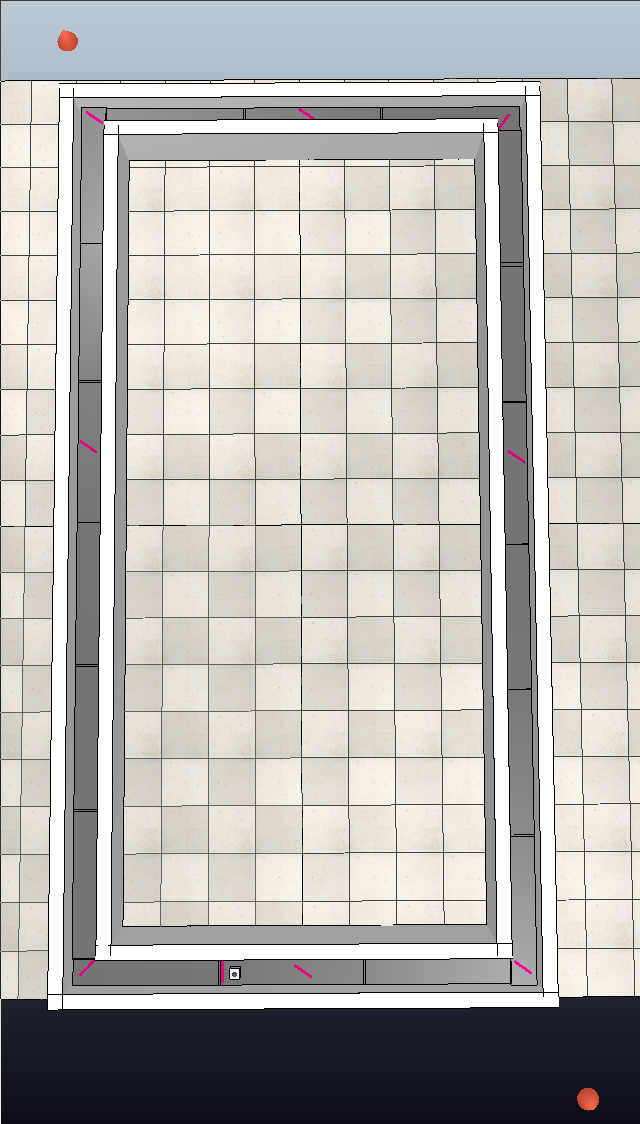
\includegraphics[angle=90, width=\linewidth]{images/long_rectangle.png}
    \caption{Modell der Route \glqq long\_rectangle\grqq\ in CoppeliaSim.}
    \label{fig:long_rectangle}
\end{figure}

\begin{figure}[h!]
    \centering
    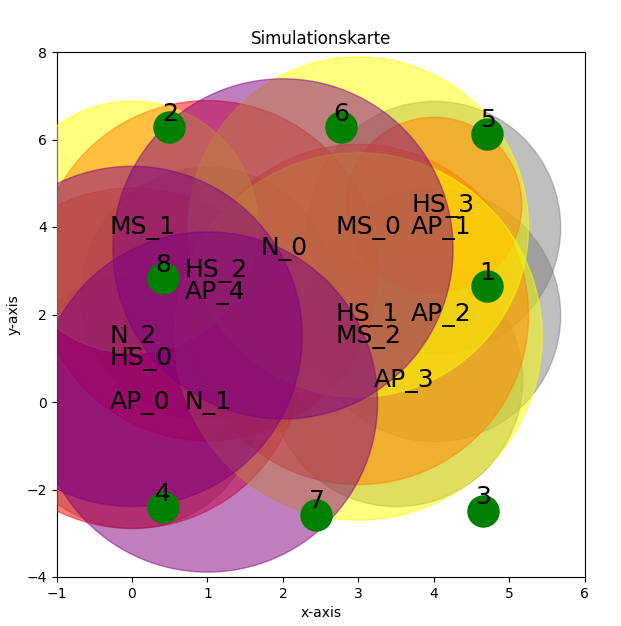
\includegraphics[width=0.9\linewidth]{images/long_rectangle_simulation_map.png}
    \caption{Karte der Route \glqq long\_rectangle\grqq\ mit eingezeichneten Einflussbereichen der Objekte, die Einfluss auf modellierte Sensoren haben.
    \textit{\textbf{M}agnetic \textbf{S}ource} (Gelb), \textit{\textbf{N}oise Source} (Lila), \textit{\textbf{A}ccess \textbf{P}oint} (Grau),
    \textit{\textbf{H}eat \textbf{S}ource} (Rot) und Standorte (Grün).}
    \label{fig:long_rectangle_simulation_map}
\end{figure}

\begin{figure}[h!]
    \centering
    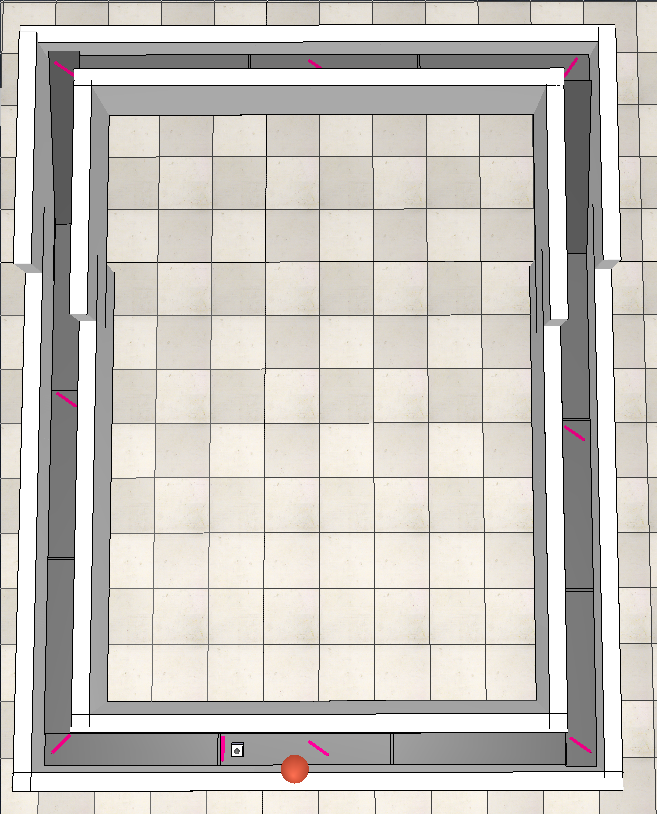
\includegraphics[angle=90, width=\linewidth]{images/rectangle_with_ramp.png}
    \caption{Modell der Route \glqq rectangle\_with\_ramp\grqq\ in CoppeliaSim.}
    \label{fig:rectangle_with_ramp}
\end{figure}

\begin{figure}[h!]
    \centering
    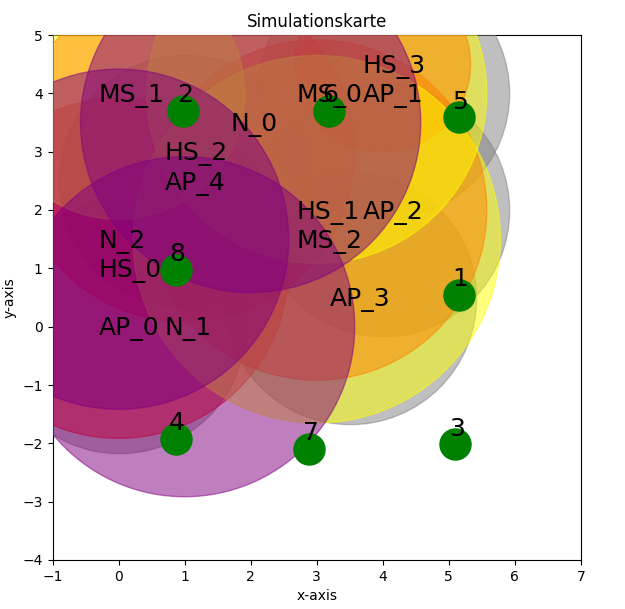
\includegraphics[width=0.9\linewidth]{images/rectangle_with_ramp_simulation_map.png}
    \caption{Karte der Route \glqq rectangle\_with\_ramp\grqq\ mit eingezeichneten Einflussbereichen der Objekte, die Einfluss auf modellierte Sensoren haben.
    \textit{\textbf{M}agnetic \textbf{S}ource} (Gelb), \textit{\textbf{N}oise Source} (Lila), \textit{\textbf{A}ccess \textbf{P}oint} (Grau),
    \textit{\textbf{H}eat \textbf{S}ource} (Rot) und Standorte (Grün).}
    \label{fig:rectangle_with_ramp_simulation_map}
\end{figure}

\begin{figure}[h!]
    \centering
    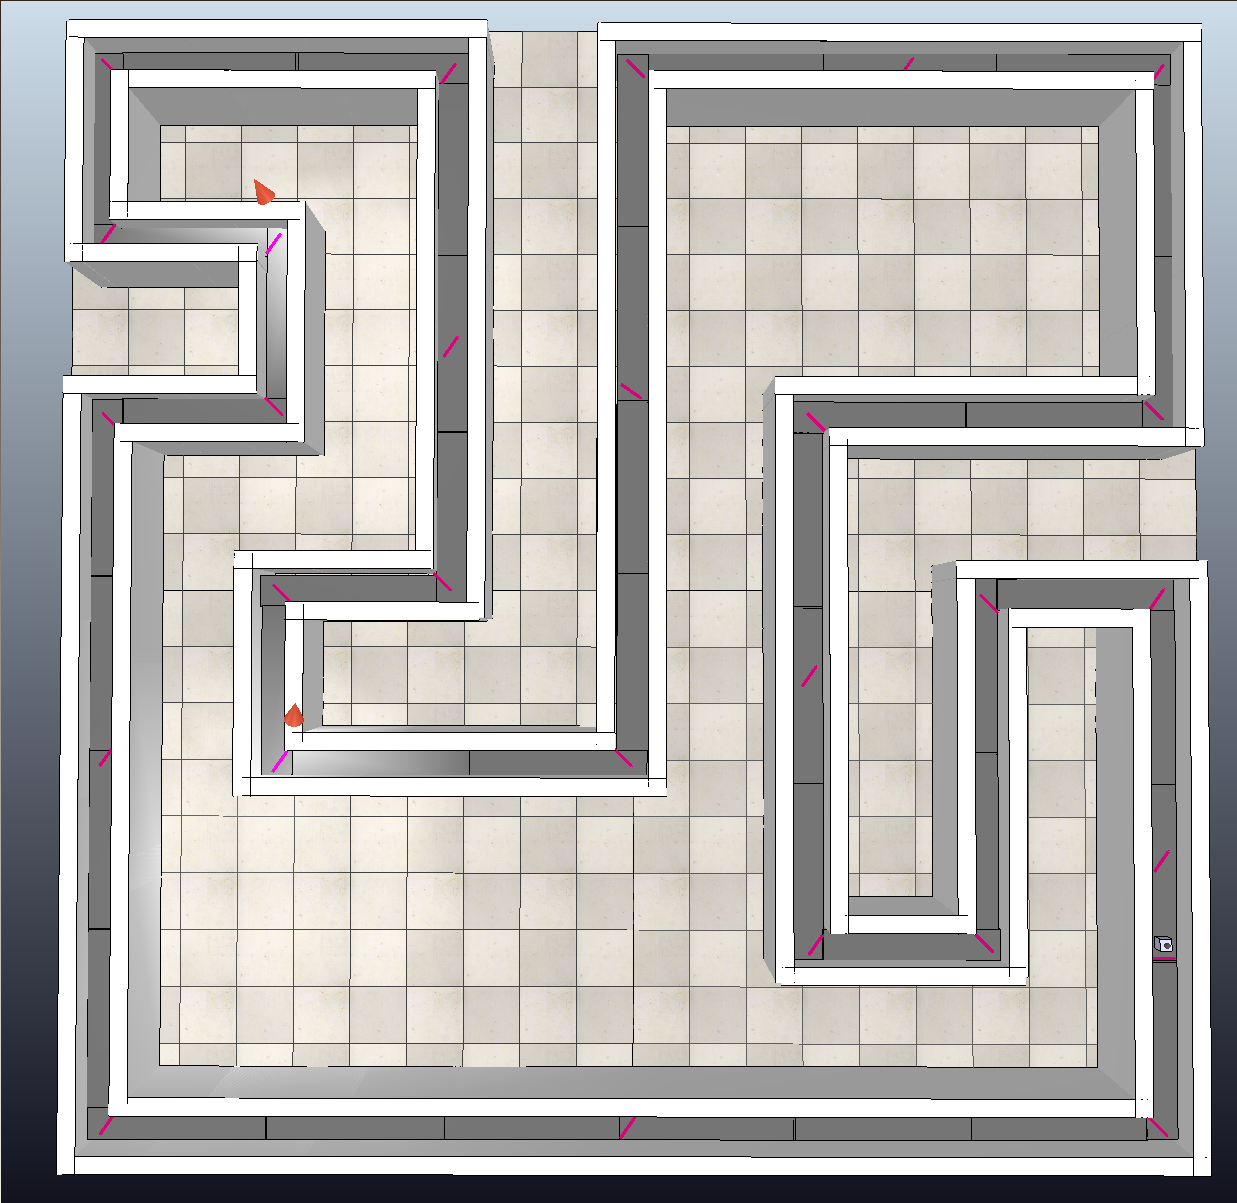
\includegraphics[width=\linewidth]{images/many_corners.png}
    \caption{Modell der Route \glqq many\_corners\grqq\ in CoppeliaSim.}
    \label{fig:many_corners}
\end{figure}

\begin{figure}[h!]
    \centering
    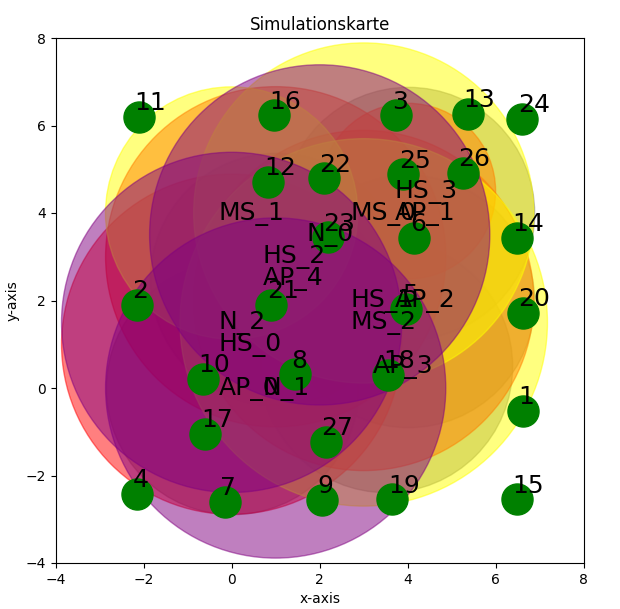
\includegraphics[width=0.9\linewidth]{images/many_corners_simulation_map.png}
    \caption{Karte der Route \glqq many\_corners\grqq\ mit eingezeichneten Einflussbereichen der Objekte, die Einfluss auf modellierte Sensoren haben.
    \textit{\textbf{M}agnetic \textbf{S}ource} (Gelb), \textit{\textbf{N}oise Source} (Lila), \textit{\textbf{A}ccess \textbf{P}oint} (Grau),
    \textit{\textbf{H}eat \textbf{S}ource} (Rot) und Standorte (Grün).}
    \label{fig:many_corners_simulation_map}
\end{figure}

\begin{figure}[h!]
    \centering
    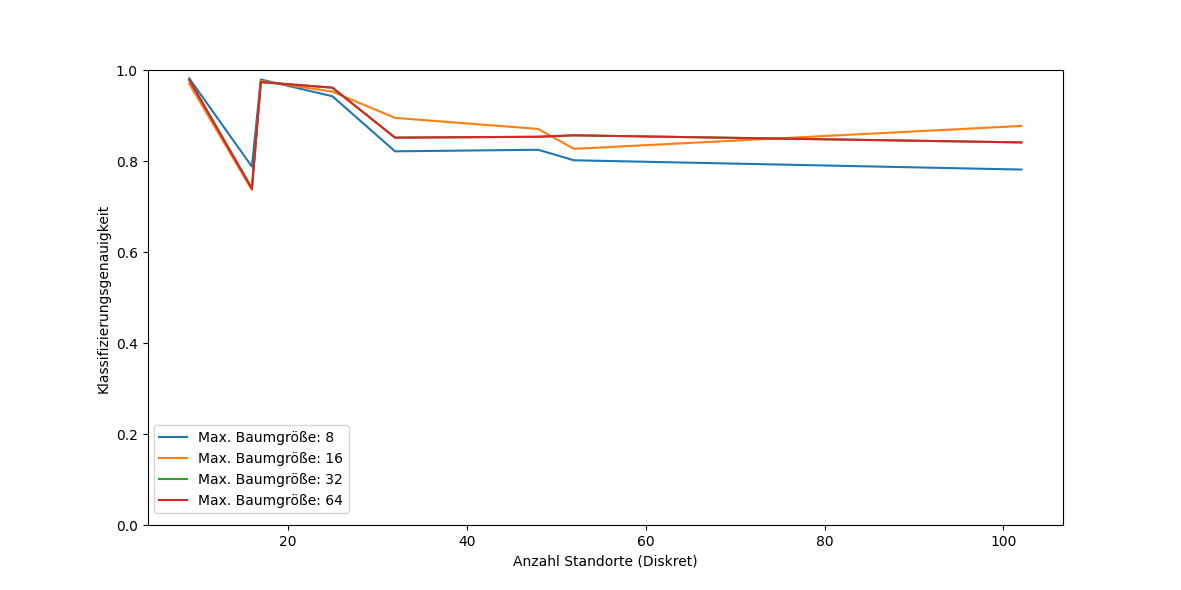
\includegraphics[width=\linewidth]{images/multiple_best_by_group_dt_max_depth_acc_5_cont.png}
    \caption{Klassifizierungsgenauigkeiten $P(B=5)$ von Entscheidungsbaum basierten Klassifizierer mit einer Waldgröße von 16 über alle Standortkomplexitäten.}
    \label{fig:multiple_best_by_group_dt_max_depth_acc_5_cont}
\end{figure}

\begin{figure}[h!]
    \centering
    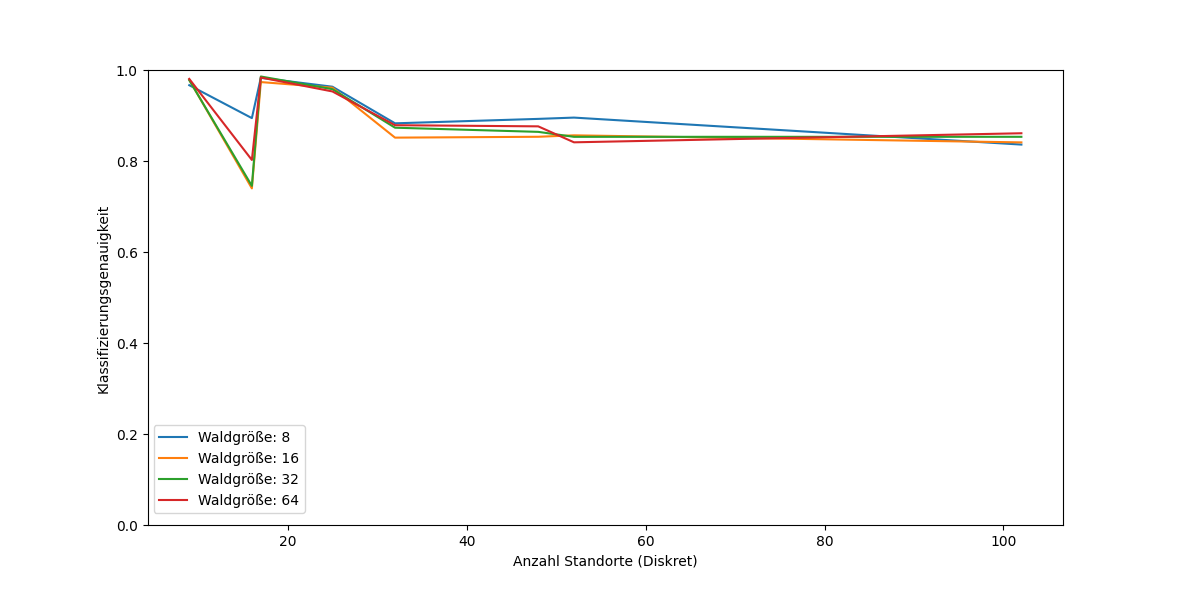
\includegraphics[width=\linewidth]{images/multiple_best_by_group_dt_trees_acc_5_cont.png}
    \caption{Klassifizierungsgenauigkeiten $P(B=5)$ von Entscheidungsbaum basierten Klassifizierer mit einer maximalen Baumhöhe von 32 über alle Standortkomplexitäten.}
    \label{fig:multiple_best_by_group_dt_trees_acc_5_cont}
\end{figure}

\begin{figure}[h!]
    \centering
    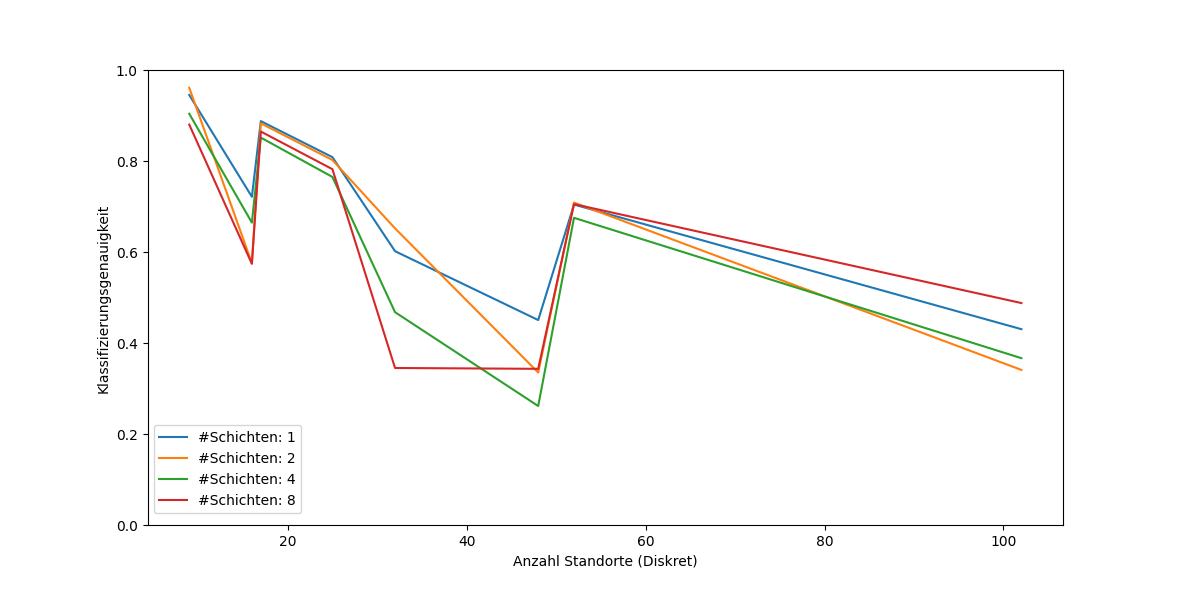
\includegraphics[width=\linewidth]{images/multiple_best_by_group_knn_layers_acc_5_cont.png}
    \caption{Klassifizierungsgenauigkeiten $P(B=5)$ von Entscheidungsbaum basierten Klassifizierer mit 32 Neuronen pro verdeckte Schicht über alle Standortkomplexitäten.}
    \label{fig:multiple_best_by_group_knn_layers_acc_5_cont}
\end{figure}

\begin{figure}[h!]
    \centering
    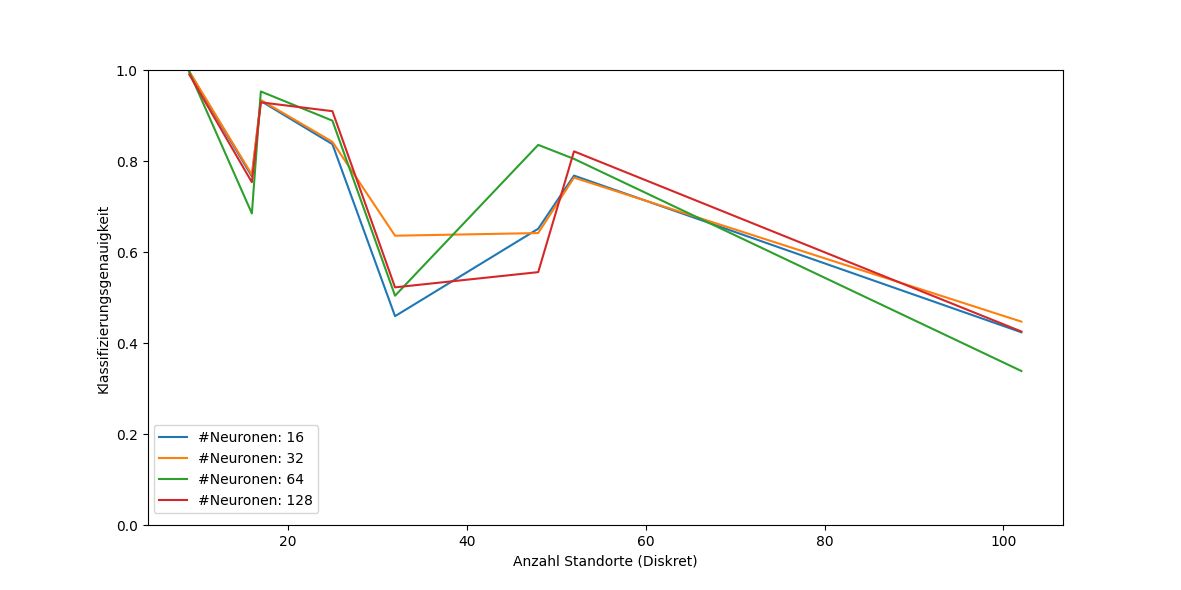
\includegraphics[width=\linewidth]{images/multiple_best_by_group_knn_neurons_acc_10_cont.png}
    \caption{Klassifizierungsgenauigkeiten $P(B=5)$ von Entscheidungsbaum basierten Klassifizierer mit einer verdeckte Schicht über alle Standortkomplexitäten.}
    \label{fig:multiple_best_by_group_knn_neurons_acc_5_cont}
\end{figure}
  \chapter{Tabellenanhänge}

\begin{table}[h!]
    \hspace{-1.5cm}
    \begin{tabular}{ | c | c | c | c | c | c | c | c | c | c | }
        \hline
        \multicolumn{2}{ | l |}{$P(A)$ über Standorte} & 9 & 16 & 17 & 25 & 32 & 48 & 52 & 102 \\\hline
        \multicolumn{10}{| l |}{\textbf{Entscheidungswälder}}\\\hline
        Waldgröße & Max. Baumgröße & \multicolumn{8}{ c |}{}\\\hline
        16 & 8 & 98.41 & 99.16\% & 98.16\% & 97.11\% & 96.47\% & 92.91\% & 95.23\% & 88.95\% \\\hline
        16 & 16 & 98.76 & 99.81\% & 98.41\% & 98.47\% & 98.87\% & 97.19\% & 98.22\% & 98.25\% \\\hline
        16 & 32 & 98.73 & 99.90\% & 98.43\% & 98.44\% & 98.74\% & 97.23\% & 98.28\% & 98.31\% \\\hline
        16 & 64 & 98.73 & 99.90\% & 98.43\% & 98.44\% & 98.74\% & 97.23\% & 98.28\% & 98.31\% \\\hline
        8 & 32 & 98.53 & 99.65\% & 98.25\% & 98.18\% & 98.62\% & 96.97\% & 97.90\% & 97.82\% \\\hline
        16 & 32 & 98.73 & 99.90\% & 98.43\% & 98.44\% & 98.74\% & 97.23\% & 98.28\% & 98.31\% \\\hline
        32 & 32 & 98.80 & 99.85\% & 98.38\% & 98.49\% & 98.90\% & 97.43\% & 98.07\% & 98.41\% \\\hline
        64 & 32 & 98.77 & 99.85\% & 98.46\% & 98.64\% & 98.73\% & 97.72\% & 98.14\% & 98.63\% \\\hline
        32 & 64 & 98.80 & 99.85\% & 98.38\% & 98.49\% & 98.90\% & 97.43\% & 98.07\% & 98.41\% \\\hline
        \multicolumn{10}{| l |}{\textbf{Feed Forward neuronale Netzwerke}}\\\hline
        \#Schichten & \#Neuronen & \multicolumn{8}{ c |}{}\\\hline
        1 & 16 & 97.96 & 98.90\% & 96.99\% & 97.28\% & 96.94\% & 89.39\% & 95.31\% & 91.73\% \\\hline
        1 & 32 & 98.27 & 99.75\% & 97.32\% & 97.54\% & 97.18\% & 93.55\% & 96.56\% & 94.19\% \\\hline
        1 & 64 & 98.41 & 99.79\% & 97.78\% & 97.88\% & 98.38\% & 95.13\% & 97.51\% & 95.39\% \\\hline
        1 & 128 & 98.29 & 99.67\% & 97.06\% & 97.79\% & 98.50\% & 95.19\% & 97.42\% & 96.47\% \\\hline
        2 & 32 & 97.69 & 99.68\% & 97.34\% & 97.88\% & 98.43\% & 94.71\% & 96.69\% & 95.30\% \\\hline
        4 & 32 & 98.10 & 99.75\% & 95.32\% & 97.85\% & 98.44\% & 95.01\% & 97.17\% & 96.96\% \\\hline
        8 & 32 & 97.30 & 99.52\% & 97.68\% & 97.79\% & 98.24\% & 94.72\% & 97.56\% & 96.39\% \\\hline
        4 & 64 & 98.24 & 99.87\% & 97.81\% & 98.31\% & 98.73\% & 94.93\% & 97.23\% & 97.26\% \\\hline
    \end{tabular}
    \caption{Metrik $P(A)$ über Standorte und verschiedenen Konfigurationen der ML-Modelle.}
    \label{tab:predictions_by_acc}
\end{table}


\begin{table}[h!]
    \hspace{-1.5cm}
    \begin{tabular}{ | c | c | c | c | c | c | c | c | c | c | }
        \hline
        \multicolumn{2}{ | l |}{$P(A)_{\text{cont}}$ über Standorte} & 9 & 16 & 17 & 25 & 32 & 48 & 52 & 102 \\\hline
        \multicolumn{10}{| l |}{\textbf{Entscheidungswälder}}\\\hline
        Waldgröße & Max. Baumgröße & \multicolumn{8}{ c |}{}\\\hline
        16 & 8 & 91.91 & 73.56\% & 93.56\% & 81.85\% & 79.88\% & 84.72\% & 75.13\% & 75.68\% \\\hline
        16 & 16 & 95.14 & 68.49\% & 95.15\% & 86.83\% & 85.56\% & 89.59\% & 81.66\% & 84.37\% \\\hline
        16 & 32 & 94.87 & 69.36\% & 95.86\% & 92.55\% & 81.69\% & 89.20\% & 82.98\% & 81.01\% \\\hline
        16 & 64 & 94.87 & 69.36\% & 95.86\% & 92.55\% & 81.69\% & 89.20\% & 82.98\% & 81.01\% \\\hline
        8 & 32 & 94.07 & 83.52\% & 95.11\% & 92.37\% & 83.76\% & 88.69\% & 81.33\% & 80.20\% \\\hline
        16 & 32 & 94.87 & 69.36\% & 95.86\% & 92.55\% & 81.69\% & 89.20\% & 82.98\% & 81.01\% \\\hline
        32 & 32 & 95.09 & 68.85\% & 95.00\% & 91.46\% & 83.79\% & 89.78\% & 81.27\% & 81.89\% \\\hline
        64 & 32 & 94.54 & 73.89\% & 95.57\% & 91.21\% & 83.75\% & 89.99\% & 77.99\% & 82.59\% \\\hline
        32 & 64 & 95.09 & 68.85\% & 95.00\% & 91.46\% & 83.79\% & 89.78\% & 81.27\% & 81.89\% \\\hline
        \multicolumn{10}{| l |}{\textbf{Feed Forward neuronale Netzwerke}}\\\hline
        \#Schichten & \#Neuronen & \multicolumn{8}{ c |}{}\\\hline
        1 & 16 & 92.20 & 63.61\% & 84.29\% & 73.19\% & 39.00\% & 60.81\% & 65.51\% & 37.72\% \\\hline
        1 & 32 & 92.11 & 63.94\% & 85.60\% & 75.38\% & 54.72\% & 60.05\% & 65.77\% & 40.17\% \\\hline
        1 & 64 & 92.54 & 55.45\% & 88.11\% & 82.39\% & 43.84\% & 78.73\% & 70.23\% & 30.75\% \\\hline
        1 & 128 & 94.71 & 61.82\% & 86.58\% & 83.63\% & 45.12\% & 52.50\% & 74.54\% & 38.74\% \\\hline
        2 & 32 & 93.30 & 48.69\% & 88.71\% & 78.63\% & 59.44\% & 68.04\% & 67.98\% & 31.87\% \\\hline
        4 & 32 & 91.13 & 58.53\% & 85.33\% & 82.58\% & 42.38\% & 48.84\% & 72.31\% & 33.77\% \\\hline
        8 & 32 & 85.51 & 50.21\% & 78.91\% & 77.75\% & 31.70\% & 66.25\% & 63.27\% & 45.04\% \\\hline
        4 & 64 & 92.60 & 54.46\% & 84.17\% & 87.28\% & 46.46\% & 44.39\% & 71.94\% & 42.34\% \\\hline
    \end{tabular}
    \caption{Metrik $P(A)_{\text{cont}}$ über Standorte und verschiedenen Konfigurationen der ML-Modelle.}
    \label{tab:predictions_by_acc_cont}
\end{table}

\begin{table}[h!]
    \hspace{-1.5cm}
    \begin{tabular}{ | c | c | c | c | c | c | c | c | c | c | }
        \hline
        \multicolumn{2}{ | l |}{$P(D)_{\text{cont}}$ über Standorte} & 9 & 16 & 17 & 25 & 32 & 48 & 52 & 102 \\\hline
        \multicolumn{10}{| l |}{\textbf{Entscheidungswälder}}\\\hline
        Waldgröße & Max. Baumgröße & \multicolumn{8}{ c |}{}\\\hline
        16 & 8 & 14.16 & 5.94\% & 20.50\% & 7.52\% & 12.34\% & 10.35\% & 10.94\% & 8.84\% \\\hline
        16 & 16 & 22.84 & 5.04\% & 23.86\% & 15.55\% & 12.65\% & 15.92\% & 10.25\% & 11.74\% \\\hline
        16 & 32 & 21.98 & 5.27\% & 26.16\% & 16.56\% & 13.66\% & 14.16\% & 11.50\% & 10.38\% \\\hline
        16 & 64 & 21.98 & 5.27\% & 26.16\% & 16.56\% & 13.66\% & 14.16\% & 11.50\% & 10.38\% \\\hline
        8 & 32 & 19.47 & 11.67\% & 24.68\% & 17.56\% & 13.29\% & 17.80\% & 10.28\% & 12.34\% \\\hline
        16 & 32 & 21.98 & 5.27\% & 26.16\% & 16.56\% & 13.66\% & 14.16\% & 11.50\% & 10.38\% \\\hline
        32 & 32 & 22.82 & 5.04\% & 21.09\% & 15.62\% & 12.01\% & 14.35\% & 11.28\% & 10.78\% \\\hline
        64 & 32 & 20.99 & 7.27\% & 23.74\% & 14.58\% & 14.35\% & 16.08\% & 10.81\% & 10.55\% \\\hline
        32 & 64 & 22.82 & 5.04\% & 21.09\% & 15.62\% & 12.01\% & 14.35\% & 11.28\% & 10.78\% \\\hline
        \multicolumn{10}{| l |}{\textbf{Feed Forward neuronale Netzwerke}}\\\hline
        \#Schichten & \#Neuronen & \multicolumn{8}{ c |}{}\\\hline
        1 & 16 & 22.20 & 5.66\% & 12.35\% & 6.74\% & 4.73\% & 6.00\% & 4.41\% & 4.00\% \\\hline
        1 & 32 & 21.23 & 6.50\% & 13.62\% & 7.59\% & 5.71\% & 6.83\% & 5.63\% & 2.66\% \\\hline
        1 & 64 & 20.52 & 5.20\% & 13.46\% & 10.40\% & 3.57\% & 9.53\% & 5.04\% & 1.74\% \\\hline
        1 & 128 & 27.11 & 5.82\% & 13.74\% & 10.66\% & 3.28\% & 3.39\% & 8.08\% & 2.57\% \\\hline
        2 & 32 & 27.28 & 4.50\% & 15.04\% & 7.86\% & 5.37\% & 4.55\% & 5.86\% & 1.74\% \\\hline
        4 & 32 & 18.24 & 5.76\% & 11.66\% & 7.27\% & 3.17\% & 2.49\% & 5.81\% & 1.77\% \\\hline
        8 & 32 & 12.61 & 3.72\% & 9.41\% & 7.15\% & 2.67\% & 3.68\% & 4.79\% & 2.71\% \\\hline
        4 & 64 & 20.21 & 5.11\% & 9.75\% & 10.49\% & 3.51\% & 1.59\% & 5.58\% & 3.99\% \\\hline
    \end{tabular}
    \caption{Metrik $P(D)_{\text{cont}}$ über Standorte und verschiedenen Konfigurationen der ML-Modelle.}
    \label{tab:predictions_by_acc_pic_cont}
\end{table}

\begin{table}[h!]
    \hspace{-1.5cm}
    \begin{tabular}{ | c | c | c | c | c | c | c | c | c | c | }
        \hline
        \multicolumn{2}{ | l |}{$P(A)$ über Standorte} & 9 & 16 & 17 & 25 & 32 & 48 & 52 & 102 \\\hline
        \multicolumn{10}{| l |}{\textbf{Entscheidungswälder}}\\\hline
        Waldgröße & Max. Baumgröße & \multicolumn{8}{ c |}{}\\\hline
        16 & 8 & 93.73\% & 90.41\% & 94.46\% & 92.75\% & 86.79\% & 81.65\% & 84.48\% & 69.10\% \\\hline
        16 & 16 & 96.10\% & 93.45\% & 96.01\% & 94.98\% & 92.20\% & 88.22\% & 88.56\% & 84.72\% \\\hline
        16 & 32 & 96.37\% & 93.71\% & 96.25\% & 94.94\% & 92.01\% & 88.07\% & 88.90\% & 84.05\% \\\hline
        16 & 64 & 96.37\% & 93.71\% & 96.25\% & 95.05\% & 92.01\% & 88.46\% & 88.91\% & 83.99\% \\\hline
        8 & 32 & 95.74\% & 93.34\% & 96.01\% & 95.20\% & 91.60\% & 88.18\% & 89.27\% & 84.48\% \\\hline
        16 & 32 & 96.37\% & 93.71\% & 96.25\% & 94.94\% & 92.01\% & 88.07\% & 88.90\% & 84.05\% \\\hline
        32 & 32 & 96.42\% & 94.18\% & 96.48\% & 95.16\% & 92.18\% & 88.89\% & 89.05\% & 85.58\% \\\hline
        64 & 32 & 96.50\% & 94.29\% & 96.47\% & 95.12\% & 92.48\% & 89.05\% & 88.97\% & 86.11\% \\\hline
        32 & 64 & 96.42\% & 94.18\% & 96.49\% & 95.09\% & 92.18\% & 88.93\% & 89.12\% & 85.61\% \\\hline
        \multicolumn{10}{| l |}{\textbf{Feed Forward neuronale Netzwerke}}\\\hline
        \#Schichten & \#Neuronen & \multicolumn{8}{ c |}{}\\\hline
        1 & 16 & 93.22\% & 84.16\% & 90.86\% & 90.77\% & 72.62\% & 74.87\% & 81.57\% & 67.42\% \\\hline
        1 & 32 & 93.06\% & 87.93\% & 91.53\% & 91.34\% & 75.69\% & 78.86\% & 82.61\% & 71.22\% \\\hline
        1 & 64 & 92.72\% & 88.50\% & 93.32\% & 91.78\% & 78.55\% & 79.05\% & 85.16\% & 72.38\% \\\hline
        1 & 128 & 93.53\% & 88.92\% & 93.46\% & 92.36\% & 81.81\% & 81.53\% & 84.87\% & 73.25\% \\\hline
        2 & 32 & 93.46\% & 88.81\% & 92.87\% & 91.55\% & 82.10\% & 79.53\% & 84.86\% & 71.41\% \\\hline
        4 & 32 & 92.21\% & 88.70\% & 92.65\% & 90.64\% & 81.34\% & 77.67\% & 84.39\% & 70.27\% \\\hline
        8 & 32 & 94.16\% & 88.48\% & 91.03\% & 91.93\% & 77.98\% & 77.17\% & 84.42\% & 70.35\% \\\hline
        4 & 64 & 93.01\% & 88.29\% & 93.35\% & 92.44\% & 82.54\% & 79.95\% & 84.82\% & 71.81\% \\\hline
    \end{tabular}
    \caption{Metrik $P(A)$ über Standorte und verschiedenen Konfigurationen der ML-Modelle ohne Rückwärtskante.}
    \label{tab:predictions_wo_feedback_edge_by_acc}
\end{table}

\end{tuhhappendix}

% Bibliography
\tuhhbibliography{thesis}

% The End
\end{document}
